% !TEX program = latexmk
% !TEX options = -lualatex -synctex=1 -interaction=nonstopmode -file-line-error "%DOC%"
\documentclass{amsart}
\usepackage{amsmath}
\usepackage{amssymb}
\usepackage{amsthm}
%\usepackage{MnSymbol}
\usepackage{bm}
\usepackage{accents}
\usepackage{mathtools}
\usepackage{tikz}
\usetikzlibrary{calc}
\usetikzlibrary{decorations.pathmorphing,shapes}
\usetikzlibrary{automata,positioning}
\usetikzlibrary{arrows.meta, shapes.geometric}
\usetikzlibrary{decorations.markings, fit}
\usepackage{tikz-cd}
\usepackage{forest} 
\usepackage{listings}
\usepackage{mdframed}
\usepackage{verbatim}
\usepackage{physics2}
\usephysicsmodule{ab,ab.legacy,diagmat,xmat,braket,op.legacy}
\usepackage{derivative}
\usepackage{fixdif}
\usepackage{stmaryrd}
% \usepackage{euscript} 
% \usepackage[mathcal]{eucal}
\usepackage{stackengine} 
%\usepackage{/home/patrickl/homework/macaulay2}

%font
% \usepackage[sc]{mathpazo}
% \usepackage{inconsolata}
\usepackage{microtype}
\usepackage{fontspec}

\setmainfont[Numbers=OldStyle]{TeX Gyre Pagella}
\setsansfont{Optima}
\usepackage{unicode-math}
\setmathfont{Asana Math}
\defaultfontfeatures{Scale=MatchLowercase}


%CS packages
\usepackage{algorithmicx}
\usepackage{algpseudocode}
\usepackage{algorithm}

% typeset and bib
\usepackage[english]{babel} 
% \usepackage[utf8]{inputenc} 
% \usepackage[T1]{fontenc}
% \usepackage[backend=biber,style=alphabetic,maxalphanames=4,maxnames=5,hyperref]{biblatex}
\usepackage[bookmarks, colorlinks, breaklinks]{hyperref} 
\hypersetup{linkcolor=blue,citecolor=magenta,filecolor=black,urlcolor=blue}
\usepackage{cleveref}
\usepackage{graphicx}
\graphicspath{{./}}
\usepackage{subcaption}
\usepackage[shortcuts]{extdash}


% other formatting packages
\usepackage{float}
\usepackage{booktabs}
\usepackage[shortlabels]{enumitem}
\setitemize{noitemsep}
\usepackage{csquotes}
%\usepackage{titlesec}
%\usepackage{titling}
%\usepackage{fancyhdr}
%\usepackage{lastpage}
% \usepackage{parskip} 
\newlist{mydescription}{description}{1}
\setlist[mydescription]{style=nextline,
                        font=\bfseries,
                        % Tweak the next 4 options as needed:
                        labelindent=1cm, 
                        leftmargin =2cm,
                        rightmargin=1cm,
                        topsep     =1ex
                       }

\usepackage{lipsum}

% delimiters
\DeclarePairedDelimiter{\gen}{\langle}{\rangle}
\DeclarePairedDelimiter{\floor}{\lfloor}{\rfloor}
\DeclarePairedDelimiter{\ceil}{\lceil}{\rceil}


\newtheorem{thm}{Theorem}[section]
\newtheorem{cor}[thm]{Corollary}
\newtheorem{prop}[thm]{Proposition}
\newtheorem{lem}[thm]{Lemma}
\newtheorem{conj}[thm]{Conjecture}
\newtheorem{quest}[thm]{Question}
\newtheorem{claim}[thm]{Claim}

\theoremstyle{definition}
\newtheorem{defn}[thm]{Definition}
\newtheorem{defns}[thm]{Definitions}
\newtheorem{con}[thm]{Construction}
\newtheorem{exm}[thm]{Example}
\newtheorem{exms}[thm]{Examples}
\newtheorem{notn}[thm]{Notation}
\newtheorem{notns}[thm]{Notations}
\newtheorem{addm}[thm]{Addendum}
\newtheorem{exer}[thm]{Exercise}

\theoremstyle{remark}
\newtheorem{rmk}[thm]{Remark}
\newtheorem{rmks}[thm]{Remarks}
\newtheorem{warn}[thm]{Warning}
\newtheorem{sch}[thm]{Scholium}
\newtheorem{conv}[thm]{Convention}


% unnumbered theorems
\theoremstyle{plain}
\newtheorem*{thm*}{Theorem}
\newtheorem*{prop*}{Proposition}
\newtheorem*{lem*}{Lemma}
\newtheorem*{cor*}{Corollary}
\newtheorem*{conj*}{Conjecture}

% unnumbered definitions
\theoremstyle{definition}
\newtheorem*{defn*}{Definition}
\newtheorem*{exer*}{Exercise}
\newtheorem*{defns*}{Definitions}
\newtheorem*{con*}{Construction}
\newtheorem*{exm*}{Example}
\newtheorem*{exms*}{Examples}
\newtheorem*{notn*}{Notation}
\newtheorem*{notns*}{Notations}
\newtheorem*{addm*}{Addendum}


\theoremstyle{remark}
\newtheorem*{rmk*}{Remark}

% shortcuts
\newcommand{\Ima}{\mathrm{Im}}
\newcommand{\A}{\mathbb{A}}
\newcommand{\G}{\mathbb{G}}
\newcommand{\N}{\mathbb{N}}
\newcommand{\R}{\mathbb{R}}
\newcommand{\C}{\mathbb{C}}
\newcommand{\Z}{\mathbb{Z}}
\newcommand{\Q}{\mathbb{Q}}
\newcommand{\X}{\mathbb{X}}
\newcommand{\E}{\mathbb{E}}
\renewcommand{\k}{\Bbbk}
\renewcommand{\L}{\mathbb{L}}
\renewcommand{\P}{\mathbb{P}}
\newcommand{\M}{\mathcal{M}}
\newcommand{\Mbar}{\overline{\mathcal{M}}}
\newcommand{\g}{\symbffrak{g}}
\newcommand{\h}{\symbffrak{h}}
\newcommand{\n}{\symbffrak{n}}
\renewcommand{\b}{\symbffrak{b}}
\newcommand{\ep}{\varepsilon}
\newcommand*{\dt}[1]{
   \accentset{\mbox{\Huge\bfseries .}}{#1}}
%\renewcommand{\abstractname}{Official Description}
\newcommand{\mc}[1]{\mathcal{#1}}
% \newcommand{\msc}[1]{\mathscr{#1}}
\newcommand{\T}{\mathbb{T}}
\newcommand{\mf}[1]{\mathfrak{#1}}
\newcommand{\mbf}[1]{\mathbf{#1}}
\newcommand{\bv}{\mbf{v}}
\newcommand{\bq}{\mbf{q}}
\newcommand{\bp}{\mbf{p}}
\newcommand{\btau}{\bm{\tau}}
\newcommand{\mr}[1]{\mathrm{#1}}
\newcommand{\on}[1]{\operatorname{#1}}
\newcommand{\ms}[1]{\mathsf{#1}}
\newcommand{\mt}[1]{\mathtt{#1}}
\newcommand{\ol}[1]{\overline{#1}}
\newcommand{\ul}[1]{\underline{#1}}
\newcommand{\wt}[1]{\widetilde{#1}}
\newcommand{\wh}[1]{\widehat{#1}}
\renewcommand{\div}{\operatorname{div}}
\newcommand{\1}{\mathbf{1}}
\newcommand{\2}{\mathbf{2}}
\newcommand{\3}{\mathbf{3}}
\newcommand{\I}{\mathrm{I}}
\newcommand{\II}{\mr{I}\hspace{-1.3pt}\mr{I}}
\newcommand{\III}{\mr{I}\hspace{-1.3pt}\mr{I}\hspace{-1.3pt}\mr{I}}
\renewcommand{\v}{\mbf{v}}
\newcommand{\w}{\mbf{w}}
\newcommand{\bmu}{\bm{\mu}}
\newcommand{\pre}{\mr{pre}}
\newcommand{\vir}{\mr{vir}}
\newcommand{\fl}{\mr{fl}}
\newcommand{\ps}[1]{\lBrack #1 \rBrack}
\newcommand{\ls}[1]{(\!( #1 )\!)}
\newcommand{\GL}{\mr{GL}}
\newcommand{\SL}{\mr{SL}}
\newcommand{\SO}{\mr{SO}}
\newcommand{\Sp}{\mr{Sp}}
\newcommand{\gl}{\mf{gl}}
\renewcommand{\sl}{\mf{sl}}
\newcommand{\so}{\mf{so}}
\renewcommand{\sp}{\mf{sp}}
\newcommand{\dbar}{\bar{\partial}}

\DeclareMathOperator{\Der}{Der}
\DeclareMathOperator{\Tor}{Tor}
\DeclareMathOperator{\Hom}{Hom}
\DeclareMathOperator{\End}{End}
\DeclareMathOperator{\Ext}{Ext}
\DeclareMathOperator{\ad}{ad}
\DeclareMathOperator{\Ad}{Ad}
\DeclareMathOperator{\Aut}{Aut}
\DeclareMathOperator{\Rad}{Rad}
\DeclareMathOperator{\Pic}{Pic}
\DeclareMathOperator{\NS}{NS}
\DeclareMathOperator{\supp}{supp}
\DeclareMathOperator{\Supp}{Supp}
\DeclareMathOperator{\depth}{depth}
\DeclareMathOperator{\sgn}{sgn}
\DeclareMathOperator{\spec}{Spec}
\DeclareMathOperator{\Spec}{Spec}
\DeclareMathOperator{\proj}{Proj}
\DeclareMathOperator{\Proj}{Proj}
\DeclareMathOperator{\ord}{ord}
\DeclareMathOperator{\Div}{Div}
\DeclareMathOperator{\Bl}{Bl}
\DeclareMathOperator{\coker}{coker}
\DeclareMathOperator{\ev}{ev}
\DeclareMathOperator{\st}{st}
\DeclareMathOperator{\pr}{pr}
\DeclareMathOperator{\ch}{ch}
\DeclareMathOperator{\Cont}{Cont}
\DeclareMathOperator{\Sym}{Sym}
\DeclareMathOperator{\Fock}{\mc{F}ock}
\DeclareMathOperator{\Crit}{Crit}

% \addbibresource{../../notes/math.bib}

\title{Notes on the B-model}
\author{Lectures on Bilibili by Si Li \\ Notes by Patrick Lei}
\date{February 2026}
\allowdisplaybreaks

\begin{document}
    
\begin{abstract}
    These are notes taken based on the~\href{https://space.bilibili.com/510673295/lists/5119099?type=season}{Bilibili minicourse} on the B-model given by Si Li in Spring 2025 at the Chinese University of Hong Kong. The minicourse consisted of 12 lectures.
\end{abstract}

\maketitle

\tableofcontents

\section{Introduction}%
\label{sec:introduction}

The B-model has its origins in \textit{mirror symmetry}, which is a duality of two dimensional superconformal field theories (SCFTs) in physics. These describe the geometry of a mapping space from a surface \(\Sigma\) to a target space \(X\) (see~\Cref{fig:surface_to_target}). The duality gives mathematical predictions which relate symplectic geometry (the A-model) to complex geometry (the B-model).

\begin{figure}[htpb]
\begin{center}
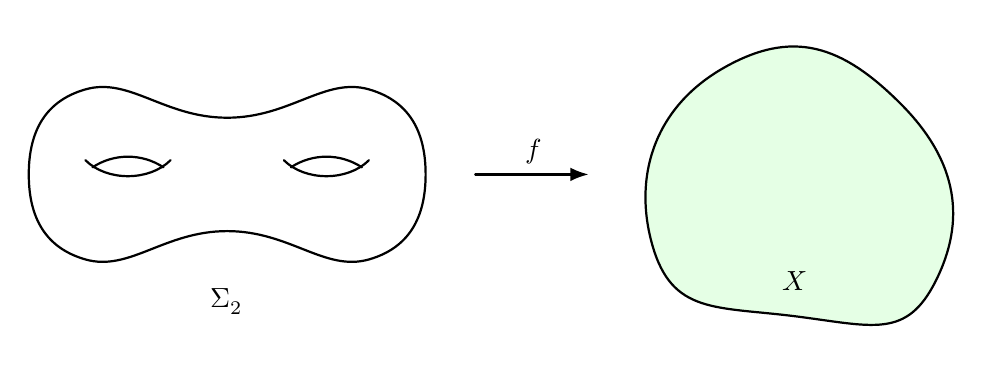
\begin{tikzpicture}[>=Latex, line cap=round, line join=round, scale=0.9]

  %--------------------------
  % Domain: Genus 2 Surface
  %--------------------------
  \begin{scope}[xshift=-4cm]
    % Main body
    \draw[thick, fill=none] plot [smooth cycle, tension=0.8] coordinates {
       (-2.8,0) (-2,1.2) (0,0.8) (2,1.2) (2.8,0) (2,-1.2) (0,-0.8) (-2,-1.2)
    };
    
    % Left Hole
    \begin{scope}[shift={(-1.4,0.1)}]
        \draw[thick] (-0.6,0.1) .. controls (-0.3,-0.2) and (0.3,-0.2) .. (0.6,0.1);
        \draw[thick] (-0.5,0) .. controls (-0.2,0.2) and (0.2,0.2) .. (0.5,0);
    \end{scope}

    % Right Hole
    \begin{scope}[shift={(1.4,0.1)}]
        \draw[thick] (-0.6,0.1) .. controls (-0.3,-0.2) and (0.3,-0.2) .. (0.6,0.1);
        \draw[thick] (-0.5,0) .. controls (-0.2,0.2) and (0.2,0.2) .. (0.5,0);
    \end{scope}

    \node at (0,-1.8) {$\Sigma_2$};
  \end{scope}

  % Map Arrow
  \draw[->, thick] (-0.5,0) -- (1.1,0) node[midway, above] {$f$};

  %--------------------------
  % Target: Space X
  %--------------------------
  \begin{scope}[xshift=4cm]
    % Blob
    \draw[thick, fill=green!10] plot [smooth cycle, tension=1] coordinates {
        (-2,-1) (-1,1.5) (1.5,1) (2,-1.5) (0,-2)
    };
    
    % Coordinate grid hint
    % \begin{scope}
    %     \clip plot [smooth cycle, tension=1] coordinates {
    %         (-2,-1) (-1,1.5) (1.5,1) (2,-1.5) (0,-2)
    %     };
    %     \draw[thin, gray!50] (-3,-3) grid (3,3);
    % \end{scope}

    \node at (0,-1.5) {$X$};
  \end{scope}

\end{tikzpicture}
\end{center}
\caption{Map from a surface \(\Sigma\) to a target space \(X\).}%
\label{fig:surface_to_target}
\end{figure}

There is a duality
\begin{equation*}
\begin{tikzcd}
    \int_{\ms{Map}(\Sigma, X)} (\text{A-model}) \ar[leftrightsquigarrow]{rr}{\text{Fourier}}[swap]{\text{T-duality}} \ar{d}[swap]{\text{localize}} & & \int_{\ms{Map}(\Sigma, X)} (\text{B-model}) \ar{d}{\text{localize}}  \\
    \int_{\ms{Hol}(\Sigma, X)} \cdots \arrow[Rightarrow]{d} & & \int_{\ms{Const}(\Sigma, X)} \cdots \arrow[Rightarrow]{d} \\
    \text{Gromov-Witten type} & & \text{Hodge-type}
\end{tikzcd}
\end{equation*}
where both sides involve some kind of infinite-dimensional geometry. However, we can reduce this to a finite-dimensional geometry by a form of supersymmetric localization, which we will not explain. The interested reader can refer to the speaker's lectures at the Perimeter Institute on supersymmetry and TQFTs, which are also on~\href{https://space.bilibili.com/510673295/lists/4795655?type=season}{Bilibili}.

There is a string description via a worldsheet theory, where we consider maps as in~\Cref{fig:worldsheet_to_target}. This theory is called \textit{string field theory}. This describes string theory using the language of quantum field theory. The correspondence goes as in~\Cref{tab:string-field-theory}.

\begin{figure}[htpb]
\begin{center}
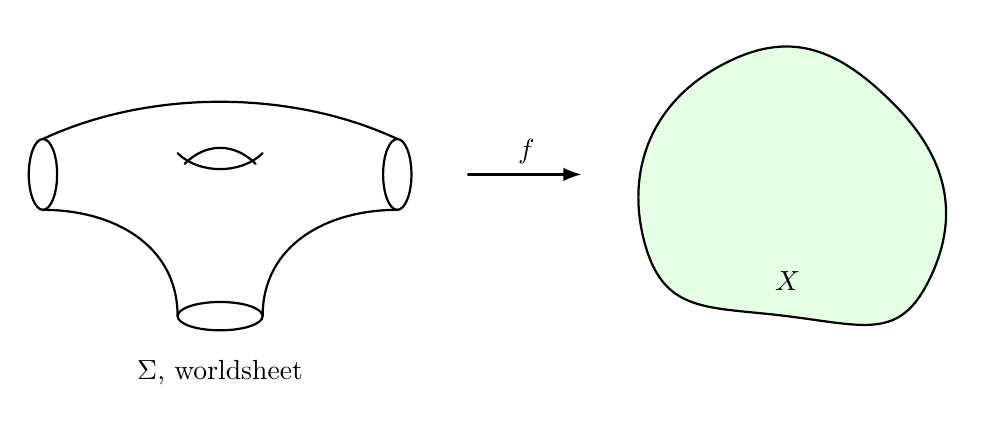
\begin{tikzpicture}[>=Latex, line cap=round, line join=round, scale=0.9]

  %--------------------------
  % Domain: Genus 1 Surface with 3 boundaries
  %--------------------------
  \begin{scope}[xshift=-4cm]
    % Top arc connecting left and right
    \draw[thick] (-2.5, 0.5) .. controls (-1, 1.2) and (1, 1.2) .. (2.5, 0.5);
    
    % Curve from left bottom to bottom left
    \draw[thick] (-2.5, -0.5) .. controls (-1.5, -0.5) and (-0.6, -1) .. (-0.6, -2);
    
    % Curve from right bottom to bottom right
    \draw[thick] (2.5, -0.5) .. controls (1.5, -0.5) and (0.6, -1) .. (0.6, -2);

    % Left cylindrical end
    \draw[thick] (-2.5, 0) ellipse (0.2 and 0.5);
    
    % Right cylindrical end
    \draw[thick] (2.5, 0) ellipse (0.2 and 0.5);

    % Bottom cylindrical end
    \draw[thick] (0, -2) ellipse (0.6 and 0.2);

    % Genus 1 Hole (Handle) - centered
    \draw[thick] (-0.6,0.3) .. controls (-0.3,0) and (0.3,0) .. (0.6,0.3);
    \draw[thick] (-0.5,0.15) .. controls (-0.2,0.45) and (0.2,0.45) .. (0.5,0.15);

    \node at (0,-2.8) {$\Sigma$, worldsheet};
  \end{scope}

  % Map Arrow
  \draw[->, thick] (-0.5,0) -- (1.1,0) node[midway, above] {$f$};

  %--------------------------
  % Target: Space X
  %--------------------------
  \begin{scope}[xshift=4cm]
    % Blob
    \draw[thick, fill=green!10] plot [smooth cycle, tension=1] coordinates {
        (-2,-1) (-1,1.5) (1.5,1) (2,-1.5) (0,-2)
    };

    \node at (0,-1.5) {$X$};
  \end{scope}

\end{tikzpicture}
\end{center}
\caption{Map in the worldsheet theory \(X\).}%
\label{fig:worldsheet_to_target}
\end{figure}


\begin{table}[htpb]
    \centering
    \caption{Idea of string field theory}
    \label{tab:string-field-theory}

    \begin{tabular}{cc}
        \toprule
        String Fock space & String field theory \\
        \midrule
        \(\ket{\psi}\) & \(\psi\) \\
        Dynamics & \(S[\psi]\) String field action \\
        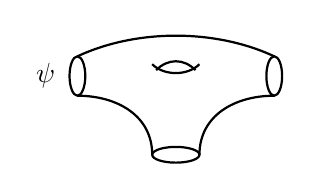
\begin{tikzpicture}[scale=0.5]
    % Top arc connecting left and right
    \draw[thick] (-2.5, 0.5) .. controls (-1, 1.2) and (1, 1.2) .. (2.5, 0.5);
    
    % Curve from left bottom to bottom left
    \draw[thick] (-2.5, -0.5) .. controls (-1.5, -0.5) and (-0.6, -1) .. (-0.6, -2);
    
    % Curve from right bottom to bottom right
    \draw[thick] (2.5, -0.5) .. controls (1.5, -0.5) and (0.6, -1) .. (0.6, -2);

    % Left cylindrical end
    \draw[thick] (-2.5, 0) ellipse (0.2 and 0.5);
    \node at (-3.3, 0) {$\ket{\psi}$};
    
    % Right cylindrical end
    \draw[thick] (2.5, 0) ellipse (0.2 and 0.5);

    % Bottom cylindrical end
    \draw[thick] (0, -2) ellipse (0.6 and 0.2);

    % Genus 1 Hole (Handle) - centered
    \draw[thick] (-0.6,0.3) .. controls (-0.3,0) and (0.3,0) .. (0.6,0.3);
    \draw[thick] (-0.5,0.15) .. controls (-0.2,0.45) and (0.2,0.45) .. (0.5,0.15);

        \end{tikzpicture} & 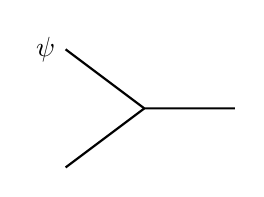
\begin{tikzpicture}[scale=0.5]
            \draw[thick] (-2,1.5) -- (0,0) -- (2.3,0);
            \draw[thick] (-2,-1.5) -- (0,0);
            \node at (-2.5,1.5) {$\psi$};
        \end{tikzpicture} \\
        \bottomrule
    \end{tabular}
\end{table}

We outline some historical developments in both mathematics and physics related to the B-model.

\begin{itemize}
    \item In 1992, Zwiebach described a general structure for closed string field theory and discovered that it is described by a string action which contains infinitely many vertices and satisfies the \textit{BV master equation}, something we will describe later in the language of the B-model. In particular, if we consider the genus \(0\) closed string field, we will discover a homotopy Lie algebra or an \(L_{\infty}\)-algebra.
    \item In 1997, Zwiebach extended this theory to the open string field, which is described by an \(A_{\infty}\)-algebra. When coupled with the closed string field, it satisfies the \textit{open-closed master equation}, which is described via the moduli of bordered Riemann surfaces.
\end{itemize}



We will consider the B-model from the perspective of string field theory. This is usually referred to as the B-twisted topological field theory, and when coupled to gravity, it becomes the topological string theory. It is localized around constant maps, and near each constant map, we see the ``local'' string field action. The correspondence goes as in~\Cref{fig:sphere_to_target}.

\begin{figure}[htpb]
\begin{center}
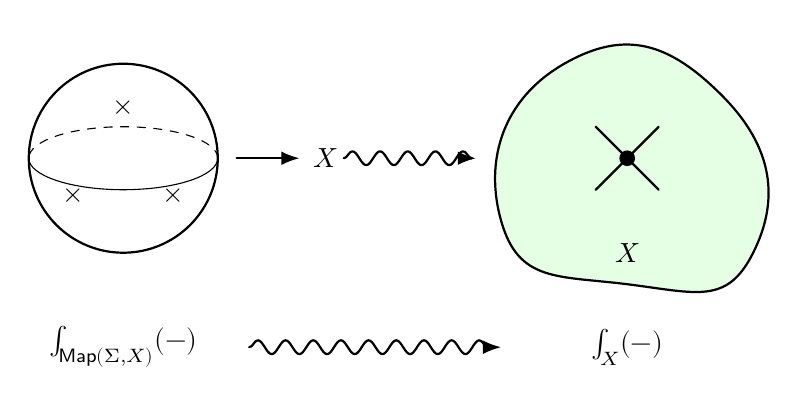
\begin{tikzpicture}[>=Latex, line cap=round, line join=round, scale=0.8, decoration=snake]

  %--------------------------
  % Domain: Sphere with 3 marked points
  %--------------------------
  \begin{scope}[xshift=-4cm]
    % Sphere
    \draw[thick] (0,0) circle (1.5);
    \draw[thin] (-1.5,0) arc (180:360:1.5 and 0.5);
    \draw[thin, dashed] (1.5,0) arc (0:180:1.5 and 0.5);

    % Marked points
    \node at (0, 0.8) {$\times$};
    \node at (-0.8, -0.6) {$\times$};
    \node at (0.8, -0.6) {$\times$};
  \end{scope}

  % Map Arrow
  \draw[->, thick] (-2.2,0) -- (-1.2,0);
  \node at (-0.8, 0) {$X$};
  \draw[->, decorate, thick] (-0.5, 0) -- (1.6,0);

  %--------------------------
  % Target: Space X
  %--------------------------
  \begin{scope}[xshift=4cm]
    % Blob
    \draw[thick, fill=green!10] plot [smooth cycle, tension=1] coordinates {
        (-2,-1) (-1,1.5) (1.5,1) (2,-1.5) (0,-2)
    };
    \node[circle, fill=black, inner sep=2pt] at (0,0) {};
    \draw[-, thick] (0,0) -- (0.5, 0.5);
    \draw[-, thick] (0,0) -- (-0.5, 0.5);
    \draw[-, thick] (0,0) -- (0.5, -0.5);
    \draw[-, thick] (0,0) -- (-0.5, -0.5);

    \node at (0,-1.5) {$X$};
  \end{scope}

  \node at (-4, -3) {$\int_{\ms{Map}(\Sigma, X)} (-)$};
  \draw[->, thick, decorate] (-2, -3) -- (2, -3);
  \node at (4, -3) {$\int_X (-)$};

\end{tikzpicture}
\end{center}
\caption{Localization of the B-model.}%
\label{fig:sphere_to_target}
\end{figure}

Here are some developments in the history of describing this new action:
\begin{itemize}
    \item Witten described the A-model open string field using Chern-Simons and instanton theories in 1992. As for the B-model open string field, he described it as holomorphic Chern-Simons theory. Finally, he speculated that the theory is actually UV-finite, which we know now is true by the work of M. Wang and J. Yan.
    \item The famous work of Bershadsky-Cecotti-Ooguri-Vafa in 1994 described the B-model closed string field theory on a Calabi-Yau threefold as a gauge theory, which they call \textit{Kodaira-Spencer gravity}. This has some interesting features:
    \begin{itemize}
        \item At the classical level, the equation of motion describes deformation of complex structures on the Calabi-Yau threefold. By Yau's proof of the Calabi conjecture, this leads to a family of solutions which are Ricci-flat metrics.
        \item The leading cubic vertex of Zwiebach's string action in the topological B-model admits a full description.
    \end{itemize}
    \item There is a construction by Barannikov-Kontsevich which constructs the Frobenius manifold (which encodes classical genus-zero data) of this theory via the geometry of polyvector fields, which will be discussed in the next few lectures.
    \item In 2012, the speaker and Kevin Costello gave a mathematical definition of the full string action for the topological B-model on a Calabi-Yau manifold of any dimension and proved that it satisfies the full BV master equation. They refer to this as \textit{BCOV theory}.
    \item In 2015/16, the same authors determined the B-model open-closed quantum coupling in the large \(N\) limit and from this perspective they worked out a version of twisted supergravity. Most of the lectures will explain the speaker's work with Costello.
\end{itemize}
    We will now fix some conventions. We will work with the category of \(\Z\)-graded vector spaces
    \[ V = \bigoplus_{m \in \Z} V_m. \]
    For any \(a \in V_m\), we will denote its degree by \(\deg(a) = \abs{a} = m\). We will denote degree shifts by
    \[ (V[n])_m = V_{m+n}, \]
    or namely, shifting to the left. Finally, we will discuss some conventions on tensors. We will denote the symmetric power by
    \[ \on{Sym}^n(V) = V^{\otimes n} / (a \otimes b \sim (-1)^{\abs{a} \abs{b}} b \otimes a) \]
    and the exterior powers by
    \[ \Lambda^n (V) = V^{\otimes n} / (a \otimes b \sim -(-1)^{\abs{a} \abs{b}} b \otimes a). \]
    These are sometimes referred to as the \textit{graded symmetric product} and the \textit{graded skew-symmetric product}. Finally, we will consider the symmetric algebra (or polynomial algebra)
    \[ \Sym(V) = \bigoplus_m \Sym^m(V) \]
    and its completion (a power series ring)
    \[ \wh{\Sym}(V) = \prod_{m} \Sym^m(V). \]
    For a graded algebra \(A\), we will always use \([-,-]\) to refer to the graded commutator, which is defined by
    \[ [a,b] = ab - (-1)^{\abs{a} \abs{b}} ba. \]
    
    Finally, if \(X\) is a smooth manifold \(X\), we will write
    \[ \Omega^{\bullet}(X) = \bigoplus_k \Omega^k (X) \]
    to denote smooth differential forms on \(X\) and denote the de Rham differential by \(\d{}\). If \(X\) is a complex manifold, we can decompose
    \[ \Omega^k(X) = \bigoplus_{p+q=k} \Omega^{p,q}(X) \]
    and decompose the differential as \(\d{} = \bar{\partial} + \partial\).


\begin{exer}
    Show that
    \[ \on{Sym}^n(V[1]) \simeq \Lambda^n(V)[n]. \]
\end{exer}

\section{Calabi-Yau geometry}%
\label{sec:Calabi-Yau geometry}

In this section, we will build some foundations for Calabi-Yau geometry. Let \(X\) be a complex manifold of dimension \(\dim_{\C} = d\). We will denote the holomorphic tangent bundle by \(T_X\). 

We will denote polyvector fields by
\[ \ms{PV}^{i,j}(X) \coloneqq \Omega^{0, j}(X, \Lambda^i T_X) \]
and the space of all polyvector fields by
\[ \ms{PV}(X) = \bigoplus_{i,j} \ms{PV}^{i,j}(X). \]
Locally, we can write \(\mu \in \ms{PV}^{i,j}(X)\) can be written as
\[ \mu = \sum_{\substack{\abs{I} = i \\ \abs{J} = j}} \mu^I_{\bar{J}} \d{\bar{z}^I} \otimes \partial_{z^I}, \]
where \(I = \{k_1, \ldots, k_i \}\) and \(J = \{ s_1, \ldots, s_j\}\) are multi-indices. Here, the index notation looks like
\[ \d{\bar{z}^J} = \d{\bar{z}^{s_1}} \wedge \cdots \wedge \d{\bar{z}^{s_j}} \qquad \text{and} \qquad \partial_{z^I} = \partial_{z^{k_1}} \wedge \cdots \wedge \partial_{z^{k_i}}. \]
These look like differential forms, but are in fact subtly different. All \(\mu^I_{\bar{J}}\) are smooth and skew-symmetric for indices in both \(I\) and in \(J\).

There is a natural (wedge) product
\[ \ms{PV}^{i_1, j_1} \otimes \ms{PV}^{i_2, j_2} \xrightarrow{\wedge} \ms{PV}^{i_1 + i_2, j_1 + j_2} \]
which makes \(\ms{PV}(X)\) a bi-graded algebra. We will define the total degree by \(\abs{\mu} = i + j\) for \(\mu \in \ms{PV}^{i,j}(X)\). This makes \((\ms{PV}(X), \wedge)\) a graded-commutative algebra, namely that \(\alpha \wedge \beta = (-1)^{\abs{\alpha} \abs{\beta}} \beta \wedge \alpha\).

We can also extend the \(\dbar\)-operator to polyvector fields, which has degree \(1\) and goes as
\[ \dbar \colon \ms{PV}^{i,j}(X) \to \ms{PV}^{i, j+1}(X). \]
This is in fact a derivation which satisfies the graded Leibniz rule
\[ \dbar (\alpha \wedge \beta) = (\dbar \alpha) \wedge \beta + (-1)^{\abs{\alpha}} \alpha \wedge \dbar \beta. \]

There are many definitions for Calabi-Yau manifolds, so we will choose one.
\begin{defn}
    A \textit{Calabi-Yau manifold} is a pair \((X, \Omega_X)\) where \(X\) is a complex manifold and \(\Omega_X\) is a nowhere-vanishing holomorphic volume form on \(X\). 
\end{defn}

In local holomorphic coordinates \(\ab\{z^1, \ldots, z^d\}\) on \(X\), we can write
\[ \Omega_X = \varphi(z) \d{z^1} \wedge \cdots \wedge \d{z^d}, \]
where \(\varphi(z)\) is a nowhere-vanishing holomorphic function. The Calabi-Yau form induces a linear isomorphism
\[ \ms{PV}^{i,j} \xrightarrow{\lrcorner \Omega_X} \Omega^{d-i, j} \qquad \mu \mapsto \mu \lrcorner \Omega_X. \]

We now consider the \textit{divergence operator}
\[ \partial_{\Omega} \colon \ms{PV}^{i,j} \to \ms{PV}^{i-1, j} \]
with respect to the volume form \(\Omega_X\), which is defined using the commutative diagram
\begin{equation*}
\begin{tikzcd}
    \ms{PV}^{i,j} \ar{d}{\sim}[swap]{\Omega_X} \ar{r}{\partial_{\Omega}} & \ms{PV}^{i-1, j} \\
    \Omega^{d-i,j} \ar{r}{\partial} & \Omega^{d-i+1, j} \ar{u}{\sim}[swap]{\Omega_X}.
\end{tikzcd}
\end{equation*}
Note that this depends on the choice of volume form. Unfortunately, we will abuse notation and write \(\partial\) for \(\partial_{\Omega}\) and whether we mean the divergence operator or the holomorphic de Rham operator will be clear from context. Unfortunately, the divergence operator is \textbf{not} a derivation. The failure is described by the tensor
\[ \ab\{\alpha, \beta \} = \partial(\alpha \wedge \beta) - (\partial \alpha) \wedge \beta - (-1)^{\abs{\alpha}} \alpha \wedge (\partial \beta). \]
This bracket is known in geometry and is related to the Schouten-Nijenhuis bracket \([-,-]_{\mr{SN}}\) by the sign
\[ [\alpha, \beta]_{\mr{SN}} = -(-1)^{\abs{\alpha}} \ab\{\alpha, \beta \}. \]
In mathematics, this is sometimes called the Bogomolov-Tian-Todorov lemma and in physics it is related to the BV algebra. In fact, the difference between the Schouten-Nijenhuis bracket and the BV bracket is related to shifting the degree by \(1\). The BV bracket has degree given by
\[ \ab\{-,-\} \colon \ms{PV}^{i_1, j_1} \otimes \ms{PV}^{i_2, j_2} \to \ms{PV}^{i_1 + i_2 - 1, j_1 + j_2}. \]
It is in fact intrinsically defined independent of the choice of volume form (or divergence operator). 

\begin{rmk}
    The lifting of \(\{-,-\}\) to the volume form \(\Omega_X\) or the divergence operator \(\partial\) is related to \textit{BV quantization}.
\end{rmk}

\begin{exer}
    Show that the BV bracket satisfies
    graded symmetry 
    \[\ab\{\alpha, \beta\} = -(-1)^{(\abs{\alpha})(\abs{\beta})} \ab\{\beta, \alpha\}, \]
    the Leibniz relation
    \[  \ab\{\alpha, \beta \wedge \gamma\} = \ab\{\alpha, \beta\} \wedge \gamma + (-1)^{\abs{\beta} \abs{\gamma}} \ab\{\alpha, \gamma\} \wedge \beta, \]
    and the graded Jacobi identity 
    \[ \ab\{ \ab\{ \alpha, \beta \}, \gamma\} = (-1)^{\abs{\alpha}} \ab\{\alpha, \ab\{\beta, \gamma\}\} - (-1)^{(\abs{\alpha}+1)\abs{\beta}} \ab\{\beta, \ab\{\alpha, \gamma\}\}. \]
\end{exer}

\begin{rmk}
    The algebra \((\ms{PV}, \dbar, \partial, \ab\{-,-\})\) is a fundamental example of a \textit{differential graded Gerstenhaber BV algebra} and exists in a large class of examples.
\end{rmk}

We can now define a \textit{trace map}
\[ \on{Tr} \colon \ms{PV}(X) \to \C \qquad \on{Tr}(\mu) \coloneqq \int_X (\mu \lrcorner \Omega_X) \wedge \Omega_X. \]
This trace is only nontrivial for \(\ms{PV}^{d,d}\) and will be used later to discuss higher residue pairings.

\begin{exer}
    Show that the trace map is compatible with the the two differentials via the identities
    \[ \on{Tr}((\dbar \alpha) \wedge \beta) = -(-1)^{\abs{\alpha}} \on{Tr}(\alpha \wedge \dbar \beta) \]
    and 
    \[ \on{Tr}((\partial \alpha) \wedge \beta) = (-1)^{\abs{\alpha}} \on{Tr}(\alpha \wedge \partial \beta). \]
\end{exer}

We will now let \(X\) be a compact Kähler manifold. The deformation space of complex structures on \(X\) is locally given by
\[ \mc{M}^{\ms{cx}} = \ab\{ \mu \in \ms{PV}^{1,1}(X) \middle\vert \norm{\mu} < \ep, \dbar \mu + \frac{1}{2} \ab\{ \mu, \mu \} = 0, \dbar^* \mu = 0\}. \]
Here, the final condition is a gauge-fixing condition and \(\dbar \mu + \frac{1}{2} \ab\{ \mu, \mu \} = 0\) is known as the \textit{Maurer-Cartan equation}.

\begin{thm}[Bogomolov-Tian-Todorov]
    Let \(X\) be a compact Kähler Calabi-Yau manifold. Then the deformation space \(\mc{M}^{\ms{cx}}\) is smooth and has dimension
    \[ \dim_{\C} \mc{M}^{\ms{cx}} = h^1(X, T_X). \]
\end{thm}

In general, we can consider the \textit{extended moduli space} \(\mc{M}\) by solving
\[ \dbar \mu + \frac{1}{2} \ab\{ \mu, \mu \} = 0 \]
modulo gauge for all types of polyvector fields. We can view the original moduli space as a submanifold of the extended one.

\begin{thm}[Barannikov-Kontsevich]
    The extended moduli space \(\mc{M}\) is smooth.
\end{thm}

\begin{proof}
    Consider the divergence-free polyvector fields \(\ker \partial \subset \ms{PV}\). Given \(\alpha, \beta \in \ker \partial\), we consider their BV bracket
    \begin{align*}
        \ab\{\alpha, \beta\} &= \partial(\alpha \wedge \beta) - (\partial \alpha) \wedge \beta - (-1)^{\abs{\alpha}} \alpha \wedge (\partial \beta) \\
        &= \partial(\alpha \wedge \beta),
    \end{align*}
    which is \(\partial\)-exact. Therefore,
    \[ \ab\{-,-\} \colon \ker \partial \otimes \ker \partial \to \Ima \partial. \]
    This fact will be crucial.

    The complex \((\ms{PV}, \dbar, \ab\{-,-\})\) is actually a (shifted) dg Lie algbera, and we consider the inclusion
    \[ j \colon (\ker \partial, \dbar, \ab\{-,-\}) \hookrightarrow (\ms{PV}, \dbar, \ab\{-,-\}). \]
    This is actually a morphism of dg Lie algebras and is in fact a quasi-isomorphism. If we allow \(\mathbb{H} \subset \ms{PV}(X)\) be the harmonic elements, then extending Hodge theory gives us
    \[ \mathbb{H} \simeq \ker \partial / \Ima \partial \simeq \ker \dbar / \Ima \dbar \]
    by the Kähler condition. Now define the projection
    \[ \Pi \colon \ker \partial \to \mathbb{H}. \]
    By the \(\partial\dbar\)-lemma, we see that \(\dbar (\ker \partial) \subset \Ima \partial\), so we can consider the map
    \[ (\ker \partial, \dbar, \{-,-\}) \xrightarrow{\Pi} (\mathbb{H}, 0, 0), \]
    which is again a morphism of dg Lie algebras. Now we have the zig-zag
    \begin{equation*}
    \begin{tikzcd}
        & (\ker \partial, \dbar, \{-,-\}) \ar[hookrightarrow]{dl}{j} \ar{dr}{\Pi} \\
        (\ms{PV}, \dbar, \{-,-\}) & & (\mathbb{H}, 0, 0),
    \end{tikzcd}
    \end{equation*}
    where both maps are quasi-isomorphisms. By some abstract nonsense, solving the Maurer-Cartan up to gauge is invariant under quasi-isomorphisms, and solving the Maurer-Cartan equation in \((\mathbb{H}, 0, 0)\) is trivial. Therefore we have \(\mc{M} \simeq \mathbb{H}\).
\end{proof}



\section{Period map}%
\label{sec:Period map}

Before we move to the B-model, we need to discuss the period map, which will allow us to write down action functionals. Let \(X, \Omega_X\) be a compact Kähler Calabi-Yau manifold. Given \(\mu \in \ms{PV}^{1,1}(X)\) satisfying the Maurer-Cartan equation
\[ \dbar \mu + \frac{1}{2} \ab\{\mu, \mu\} = 0, \]
we will use \([X_{\mu}] \in \mc{M}^{\ms{cx}}\) to denote the complex manifold specified by the deformation \(\mu\). Assume that \(\ab\{z^i\}\) are local holomorphic coordinates on \(X\). We can write
\[ \mu = \sum_{i,j} \mu_{\bar{\jmath}}^i \d{\bar{z}}^j \otimes \partial_{z^i}. \]
Then we can define new holomorphic \(1\)-forms by
\begin{align*}
    (\d{z^i} + \mu \lrcorner \d{z^i}) &= \d{z^i} + \sum_j \mu_{\bar{\jmath}}^i \d{\bar{z}}^j \\
    &= e^{\mu} \lrcorner \d{z^i},
\end{align*}
and these form a local basis of \((1,0)\)-forms on \(X_{\mu}\). 

Let \(\mc{H}^d\) denote the complex vector bundle over \(\mc{M}^{\ms{cx}}\) whose fiber at \([X_{\mu}]\) is the de Rham cohomology \(H^d(X_{\mu})\). This bundle admits a flat connection, called the \textit{Gauss-Manin connection}, and denoted by \(\nabla^{\ms{GM}}\), which identifies the nearby fibers to the central one as
\[ H^d (X_{\mu}) \simeq H^d(X). \]
There is some global issue with monodromy, but locally the identification is canonical. We now define the holomorphic subbundles (the Hodge filtration)
\(\mc{F}^p \mc{H}^d \subset \mc{H}^d\) with fibers
\[ \mc{F}^p \mc{H}^d|_{[X_{\mu}]} = \bigoplus_{k \geq p} H^{k, d-k}(X_{\mu}). \]
In particular, there is the line bundle \(L = \mc{F}^d \mc{H}^d\) which picks up the holomorphic volume form on \(X_{\mu}\). In physics, this is known as the \textit{vacuum line bundle}. Later, we will see that invariants of the B-model are actually sections of powers of this line bundle.

The period map is locally given by the map
\[ \mc{M}^{\ms{cx}} \hookrightarrow \P (H^d (X, \C)) \qquad [X_{\mu}] \mapsto [\Omega_{X_{\mu}}]. \]
Here, we need to use the Gauss-Manin connection to identify the cohomology of \(X_{\mu}\) with that of \(X\). The period map is actually a local embedding (the local Torelli theorem). Sometimes it is helpful to remember the actual volume form, and if we consider the \(\C^{\times}\)-bundle 
\[ \hat{\mc{M}}^{\ms{cx}} = \on{Tot}(L \setminus \{0\}) \]
over \(\mc{M}^{\ms{cx}}\), then a point here represents a pair \((X, \Omega_X)\), so we have defined the local moduli of deformations of a pair \((X, \Omega_X)\). This allows us to lift the period map to an embedding
\[ \hat{\mc{M}}^{\ms{cx}} \hookrightarrow H^d(X, \C) \qquad (X_{\mu}, \Omega_{X_{\mu}}) \mapsto [\Omega_{X_{\mu}}]. \]

Our goal is to understand the geometry of the period map, which will allow us to understand the action functional of the B-model. We will begin with the case of Calabi-Yau threefolds, which is classical, and then move to a more modern perspective. Let \((X, \Omega_X)\) be a Calabi-Yau threefold. Then \(H^3(X, \C)\) has a symplectic pairing given by
\[ \omega(\alpha, \beta) = \int_X \alpha \wedge \beta. \]
Considering the Hodge filtration, the subspace
\[ F^2 H^3 = H^{3,0} \oplus H^{2,1} \subset H^3 \]
is a Lagrangian subspace. Over the moduli space \(\mc{M}^{\ms{cx}}\) \(\omega\) defines a fiberwise symplectic pairing on \(\mc{H}^3\) which is flat with respect to the Gauss-Manin connection. Then we can lift the Hodge filtration to a subbundle
\[ \mc{F}^2 \mc{H}^3 \subset \mc{H}^3, \]
which gives a holomorphic family of Lagrangian subspaces. 

\begin{prop}
    The embedding \(\hat{\mc{M}}^{\ms{cx}} \hookrightarrow H^3\) defines a Lagrangian submanifold.
\end{prop}

\begin{proof}
    Let \(\Omega_s\) be a holomorphic family of Calabi-Yau forms parameterized by \(s\). By Griffiths transversality, we see that
    \[ \nabla^{\ms{GM}} \Omega_s \subset \mc{F}^2 \mc{H}^3. \]
    Every fiber is a linear Lagrangian subspace, so we are done.
\end{proof}

From this data, we can cook up B-model invariants as follows. Choose a Lagrangian splitting \(\mc{L} \subset H^3(X, \C)\) be a transversal linear Lagrangian subspace such that
\[ H^3 = F^2 H^3 \oplus \mc{L} \]
is an isotropic splitting. This allows us to identify
\[ H^3 \cong T^* F^2, \]
where we use \(F^2\) to refer to \(F^2 H^3\). Then \(\hat{\mc{M}}^{\ms{cx}}\) is a Lagrangian submanifold as in~\Cref{fig:lagrangian_submanifold}. Therefore, there is some function \(\hat{F}_0 \in \mc{O}(F^2)\) such that \(\hat{\mc{M}}^{\ms{cx}}\) is the graph of \(\d{\hat{F}_0}\). 

\begin{figure}[htpb]
\begin{center}
\begin{tikzpicture}[x=1.05cm,y=1.05cm,>=Stealth,line cap=round,line join=round]
  % white background (optional; remove if your page is already white)
  \fill[white] (-4.9,-3.6) rectangle (7.0,4.4);

  % axes
  \draw[thick,->] (-4.6,0) -- (5.4,0) node[right] {$F^2$};
  \draw[thick,->] (0,-3.2) -- (0,4.2);

  % labels
  \node at (3.9,3.45) {$H^3 \simeq T^{*}F^2$};
  \node at (4.0,1.65) {$\hat{\mathcal M}^{\mathrm{cx}}$};

  % curve
  \draw[thick]
    (-3.2,-0.8)
    .. controls (-3.0,1.3) and (-2.4,2.2) .. (-1.7,2.0)
    .. controls (-1.0,1.8) and (-0.4,0.9) .. (0,0)
    .. controls (0.5,-0.9) and (1.2,-1.4) .. (1.8,-1.1)
    .. controls (2.3,-0.8) and (2.5,-0.1) .. (2.7,0.6)
    .. controls (2.9,1.3) and (3.2,1.7) .. (3.6,1.7);
\end{tikzpicture}
\end{center}
\caption{The moduli space \(\hat{\mathcal M}^{\mathrm{cx}}\) as a Lagrangian submanifold in \(H^3 \simeq T^* F^2\).}%
\label{fig:lagrangian_submanifold}
\end{figure}

\begin{exm}
    Choose \(\mc{L} = H^{1,2} \oplus H^{0,3}\) (the complex conjugate splitting). Physicists would now write down some special geometry and prepotentials. We parametrize \(\hat{\mc{M}}^{\ms{cx}}\) by
    \[ \hat{\mc{M}}^{\ms{cx}} = \ab\{ (t^0, t^i \partial_{t^i} \hat{F}_0, \partial_{t^0} \hat{F}_0) \}. \]
    Because \(\mc{M}^{\ms{cx}} = \hat{\mc{M}}^{\ms{cx}} / \C^{\times}\), we see that \(\hat{F}_0\) has homogeneous degree \(2\). The local coordinates on \(\mc{M}^{\ms{cx}}\) are given by \(\tau^i = \frac{t^i}{t^0}\). Therefore, we can write
    \[ \hat{F}_0 = (t_0)^2 \mc{F}_0 (\tau^i). \]
    Geometrically, \(\hat{F}_0\) actually defines a local section of \(L^{\otimes -2}\), where \(L\) is the vacuum line bundle. We can now reparaterize the extended moduli space by
    \[ \hat{\mc{M}}^{\ms{cx}} = \ab\{ t^0 (1, \tau^i \partial_{\tau^i} \mc{F}_0, 2 \mc{F}_0 - \tau^i \partial_{\tau^i} \mc{F}_0) \}. \]
    The factor inside the parentheses is called the \textit{primitive period map}. We now obtain a particular choice of holomorphic volume form on the moduli space given by
    \[ [\Omega_{\tau}] = (1, \tau^i, \partial_{\tau^i} \mc{F}_0, 2 \mc{F}_0 - \tau^i \partial_{\tau^i} \mc{F}_0). \]
    We are now finally able to calculate the \textit{Yukawa coupling} for the moduli space by
    \begin{align*}
        C_{ijk}(\tau) &= \int \nabla^{\ms{GM}}_{\partial_{\tau^i}} [\Omega_{\tau}] \wedge \nabla^{\ms{GM}}_{\partial_{\tau^j}} \nabla^{\ms{GM}}_{\partial_{\tau^k}} [\Omega_{\tau}] \\
        &= \partial_{\tau^i} \partial_{\tau^j} \partial_{\tau^k} \mc{F}_0 (\tau).
    \end{align*}
    In the physics literature, \(\mc{F}_0(\tau)\) is called the \textit{prepotential}.
\end{exm}

\begin{exer}
    Prove the formula for the Yukawa coupling in the previous example.
\end{exer}

Before we proceed, we need to describe the deformation of the pair \((X, \Omega_X)\). We know that deformations of \(X\) are given by \(\mu \in \ms{PV}^{1,1}(X)\) satisfying the Maurer-Cartan equation
\[ \dbar \mu + \frac{1}{2} \ab\{\mu, \mu\}  = 0. \]
In the complex structure \(X_{\mu}\) specified by \(\mu\), the elements
\[ e^{\mu} \lrcorner \d{z^i} = \d{z^i} + \mu \lrcorner \d{z^i} \]
form a new basis of \((1,0)\)-forms on \(X_{\mu}\).

\begin{lem}
    We have
    \[ e^{\mu} \lrcorner (\alpha \wedge \beta) = (e^{\mu} \lrcorner \alpha) \wedge (e^{\mu} \lrcorner \beta) \]
    for any differential forms \(\alpha, \beta\).
\end{lem}

The lemma now implies that 
\[ e^{\mu} \lrcorner (\d{z^1} \wedge \cdots \wedge \d{z^d}) \]
is of type \((d, 0)\) with respect to \(X_{\mu}\). Applying this globally, the form
\[ e^{\mu} \lrcorner \Omega_X \]
is of type \((d, 0)\) in \(X_{\mu}\). Therefore, there exists a smooth function \(\rho\) such that
\[ e^{\rho} e^{\mu} \lrcorner \Omega_X \]
is a holomorphic volume form on \(X_{\mu}\). Because the type is \((d, 0)\), then the form is holomorphic if and only if it is closed, or in other words that \(\d{(e^{\rho} e^{\mu} \lrcorner \Omega_X)} = 0\). This gives us the two equations
\[ \begin{cases}
    \dbar \mu + \frac{1}{2} \ab\{\mu, \mu\} = 0 & \rightsquigarrow \text{deform to } X_{\mu}\\
    \dbar \rho + \partial \mu + \ab\{ \mu, \rho \} = 0 & \rightsquigarrow \text{deform to } \Omega_{X_{\mu}}
\end{cases} \]
which govern deformations of the pair \((X, \Omega_X)\). These equations were studied by Barannikov in his work on variations of semi-infinite Hodge structures.

\section{Extended period map}%
\label{sec:Extended period map}

Introduce a formal parameter \(t\) of degree \(2\), which will play the role of gravitational descendents and consider the combined differential
\[ Q = \dbar + t \partial. \]
We can rewrite our two equations as the single equation
\[ Q \hat{\mu} + \frac{1}{2} \ab\{\hat{\mu}, \hat{\mu}\} = 0, \]
where we have defined
\[ \hat{\mu} = \mu + t \rho. \]
Introduce a new (shifted) dg Lie algebra
\[ (\ms{PV}(X)\ps{t}, Q = \dbar + t \partial, \ab\{-,-\}). \]

\begin{rmk}
    The data of \((\ms{PV}(X) \ps{t}, Q)\) can be viewed as a homological replacement of volume-preserving (divergence-free) vector fields \((\ker \partial, \dbar)\). We may now write the complex
    \[ \ker \partial \to \ms{PV} \xrightarrow{t \partial} t \ms{PV} \xrightarrow{t \partial} t^2 \ms{PV} \to \cdots \]
    which behaves badly, so we replace it with \((\ms{PV} \ps{t}, Q)\).
\end{rmk}

\begin{rmk}
    The variable \(t\) plays the role of gravitational descendants (namely \(\psi\)-classes on the A-side) in the B-model.
\end{rmk}

\begin{rmk}
    If \((\ms{PV}, \dbar, \ab\{-.-\})\) gives extended moduli for \(X\), then \((\ms{PV} \ps{t}, Q, \ab\{-,-\})\) gives extended moduli for the Calabi-Yau geometry.
\end{rmk}

\begin{rmk}
    The variable \(t\) can be viewed as an equivariant parameter for rotation on the worldsheet in the worldsheet B-model.
\end{rmk}

\begin{quest}
    Can we express the above equations as the variational critical locus of some action functional?
\end{quest}

One reason we would be interested in this question is because this is the usual approach to classical physics, and then we can quantize these using path integrals. This is unfortunately highly nontrivial, and on a Calabi-Yau threefold, BCOV work with some \(\mu \in \ker \partial\). They found that the Maurer-Cartan equation
\[ \dbar \mu + \frac{1}{2} \ab\{\mu, \mu\} = 0 \]
is equivalent to \(\fdv{\ms{KS}}{\mu} = 0\) for the Kodaira-Spencer action \(\ms{KS}\).

\begin{warn}
    This approach unfortunately violates locality for various reasons:
    \begin{itemize}
        \item \(\ker \partial\) is not a module over \(C^{\infty}(X)\);
        \item One of the terms in \(\ms{KS}\) is nonlocal.
    \end{itemize}
\end{warn}

Consider the Calabi-Yau geometry and let \(\mu \in \ms{PV}(X)\ps{t}\). We can ask for an action functional whose critical points are solutions of
\[ Q \mu + \frac{1}{2} \ab\{\mu, \mu\} = 0. \]
Unfortunately, the speaker was unable to find this, but there is some magic involved. If we perform an \(L_{\infty}\) transformation, this equation becomes
\[ Q \mu + \sum_{k \geq 2} \frac{1}{k!} \ell_k (\mu^{\otimes k}) = 0, \]
and for this equation there is a BCOV action which was found by Costello and the speaker. The \(L_{\infty}\) transformation is produced directly from the period map.

\begin{defn}
    Define
    \[ \ms{S}(X) \coloneqq \ms{PV}(X) \ls{t}[2], \]
    where the shift makes \(\mu + t \rho\) have degree \(0\). Then define
    \[ \ms{S}_+(X) \coloneqq \ms{PV}(X) \ps{t}[2] \qquad \text{and} \qquad \ms{S}_-(X) \coloneqq t^{-1} \ms{PV}(X)[{t^{-1}}][2]. \]
    This makes \(\ms{S}(X) = \ms{S}_+(X) \oplus \ms{S}_-(X)\), and once we define a symplectic structure it will be a splitting by isotropic subspaces. However, \(Q\) does \textbf{not} preserve the splitting, but this will lead to the classical master equation.

    We define a \(t\)-sesquilinear pairing on \(\ms{S}(X)\) (inspired by the higher residue pairing of Kyoji Saito)
    \[ \omega \colon \ms{S}(X) \otimes \ms{S}(X) \to \C \]
    by the formula
    \[ \omega(f(t) \alpha, g(t) \beta) \coloneqq \Tr \alpha\beta \on{Res}_{t = 0} f(t) g(-t) \d{t}. \]
    Observe that
    \begin{align*}
        \omega (g(t) \beta, f(t) \alpha) &= \Tr \beta\alpha \on{Res}_{t = 0} g(t) f(-t) \d{t} \\
        &= - (-1)^{\abs{\alpha} \abs{\beta}} \Tr \alpha\beta \on{Res}_{t = 0} f(t) g(-t) \d{t} \\
        &= - (-1)^{\abs{\alpha} \abs{\beta}} \omega(f(t) \alpha, g(t) \beta).
    \end{align*}
\end{defn}

If we calculate the degrees, then \(\omega\) is only nontrivial when 
\begin{align*}
    \deg (f(t) \alpha) + \deg (g(t) \beta) &= \deg (\alpha \wedge \beta) + \deg f(t) + \deg g(t) \\
    &= 2d - 2,
\end{align*}
so if we take the original shift by \(2\) into account, we have proved the following result.

\begin{prop}
    The space \((\ms{S}(X), \omega)\) has a \((6-2d)\)-shifted symplectic structure.
\end{prop}

\begin{rmk}
    For a Calabi-Yau threefold \(X\), we have the splitting
    \[ \Omega^3 = \Omega^{3,0} \oplus \Omega^{2,1} \oplus \Omega^{1,2} \oplus \Omega^{0,3}, \]
    and the we will be able to identify this with
    \[ t \ms{PV}^{0,0} \oplus \ms{PV}^{1,1} \oplus t^{-1} \ms{PV}^{2,2} \oplus t^{-2} \ms{PV}^{3,3} \]
    via contraction with \(\Omega_X\), which we will call \(\Gamma\). The higher residue pairing will be identified with the usual pairing on differential forms. We should note however that this only works for threefolds.
\end{rmk}

\begin{prop}
    The operator \(Q\) is (graded) skew-symmetric with respect to \(\omega\).
\end{prop}

\begin{proof}
    The proof is left as an exercise. The key point is to study the operators \(\dbar\) and \(\partial\).
\end{proof}

We now consider the (cochain) period map
\[ \mc{P} \colon \ms{S}_+(X) \to \ms{S}(X) \qquad \mu \mapsto t \ab(1-e^{\mu/t}). \]

\begin{rmk}
    This \(\mc{P}\) is understood as a map on formal schemes. For any Artinian ring \((R, \mf{m})\), we send
    \[ \mu \in \ms{S}_+(X) \otimes \mf{m} \mapsto t \ab(1-e^{\mu/t}) \in \ms{S}(X) \otimes \mf{m}. \]
    This truncates at finite order, so the map is well-defined.
\end{rmk}

We compute the tangent map at \(\mu = 0\), and we see
\[ \delta \mu \mapsto t \ab(1 - e^{\delta \mu/t}) = - \delta \mu + \cdots, \]
so we see that
\[ \d{\mc{P}}_* \colon T_0 \ms{S}_+(X) = \ms{S}_+(X) \to T_0 \ms{S}(X) = \ms{S}(X) \]
is simply the inclusion with a sign of \(-1\). See~\Cref{fig:cochain-period-map} for a visualization. This implies that \(\mc{P}\) is a formal embedding.

\begin{figure}[htpb]
\begin{center}
\begin{tikzpicture}[x=0.55cm,y=0.55cm,>=Stealth,line cap=round,line join=round]
  \draw[thick, ->] (-16,0) -- (-10, 0) node[above] {$\ms{S}_+(X)$};
  \node at (-13, -0.5) {$\mu$};
  \draw[->] (-9, 0) to [bend left]  node[above] {$\mc{P}$} (-5, 0);
  % axes
  \draw[thick,->] (-4.6,0) -- (5.0,0) node[right] {$\ms{S}_+$};
  \draw[thick,->] (0,-3.2) -- (0,4.2);

  % labels
  \node at (3.9,3.45) {$\ms{S}(X)$};

  % curve
  \draw[thick]
    (-3.2,-0.8)
    .. controls (-3.0,1.3) and (-2.4,2.2) .. (-1.7,2.0)
    .. controls (-1.0,1.8) and (-0.6,0.0) .. (0,0)
    .. controls (0.6,0.0) and (1.2,-1.4) .. (1.8,-1.1)
    .. controls (2.3,-0.8) and (2.5,-0.1) .. (2.7,0.6)
    .. controls (2.9,1.3) and (3.2,1.7) .. (3.6,1.7);
\end{tikzpicture}
\end{center}
\caption{The cochain period map}%
\label{fig:cochain-period-map}
\end{figure}

This map is actually an \(L_{\infty}\)-morphism
\[ (\ms{S}_+(X), Q, \ab\{-,-\}) \xrightarrow{\mc{P}}  (\ms{S}(X), Q, 0). \]
One way to see this is to check that the Maurer-Cartan equation is preserved. We can check that 
\begin{align*}
    Q \ab(t \ab(1-e^{\mu/t})) &= -\ab(Q \mu + \frac{1}{2} \ab\{\mu, \mu\}) e^{\mu/t},
\end{align*}
and therefore we see that \(\mu\) satisfies the Maurer-Cartan equation if and only if \(\mc{P}(\mu)\) does. Therefore, if we view \(Q\) as a vector field on \(\ms{S}(X)\), then \(Q\) is tangent to \(\Ima(\mc{P})\) and is thus the pushforward of a vector field on \(\ms{S}_+(X)\) which defines the \(L_{\infty}\) structure.

The image \(\Ima(\mc{P}) \subset \ms{S}(X)\) of the period map is a formal Lagrangian submanifold. If we calculate the variation of the period map, we see that
\begin{align*}
    \delta \ab(t \ab(1-e^{\mu/t})) &= - \delta \mu e^{\mu/t} \\
    &\subset \ms{S}_+(X) e^{\mu/t}.
\end{align*}

\begin{prop}
    For all \(\alpha, \beta \in \ms{S}_+(X)\), we have
    \[ \omega \ab(\alpha e^{\mu/t}, \beta e^{\mu/t}) = 0. \]
\end{prop}

\begin{proof}
    The proof is left as an exercise.
\end{proof}

\section{Classical BCOV action}%
\label{sec:Classical BCOV action}

Some references for this include the surveys \href{https://link.springer.com/content/pdf/10.1007/978-3-319-94220-9_4.pdf}{Some classical/quantum aspects of Calabi-Yau moduli} and \href{https://sigma-journal.com/2012/101/sigma12-101.pdf}{Renormalization method and mirror symmetry} by the lecturer in addition to his work with Costello.

We will begin with a toy model to describe the geometry of gravitational descendants. Suppose the case when \(X\) is a point. In this case, \(\ms{S} = \C \ls{t}\), \(\ms{S}_+ = \C \ps{t}\), and \(\ms{S}_- = t^{-1} \C[t^{-1}]\). The symplectic pairing is given by
\[ \omega(f(t), g(t)) = \on{Res}_{t = 0} f(t) g(-t) \d{t}. \]
The period map now looks like~\Cref{fig:cochain-period-map-point}. The image of the period map is a formal Lagrangian submanifold.

\begin{figure}[htpb]
\begin{center}
\begin{tikzpicture}[x=0.55cm,y=0.55cm,>=Stealth,line cap=round,line join=round]
  \draw[thick, ->] (-16,0) -- (-10, 0) node[above] {$\ms{S}_+(X)$};
  \node at (-13, -0.5) {$f(t)$};
  \draw[->] (-9, 0) to [bend left]  node[above] {$\mc{P}$} (-5, 0);
  % axes
  \draw[thick,->] (-4.6,0) -- (5.0,0) node[right] {$\ms{S}_+$};
  \draw[thick,->] (0,-3.2) -- (0,4.2);

  % labels
  \node at (3.9,3.45) {$\ms{S} = \C \ps{t}$};

  % curve
  \draw[thick]
    (-3.2,-0.8)
    .. controls (-3.0,1.3) and (-2.4,2.2) .. (-1.7,2.0)
    .. controls (-1.0,1.8) and (-0.6,0.0) .. (0,0)
    .. controls (0.6,0.0) and (1.2,-1.4) .. (1.8,-1.1)
    .. controls (2.3,-0.8) and (2.5,-0.1) .. (2.7,0.6)
    .. controls (2.9,1.3) and (3.2,1.7) .. (3.6,1.7);
    \node at (-1.8, 2.5) {$t(1-e^{f/t})$};
\end{tikzpicture}
\end{center}
\caption{The cochain period map for \(X = \mr{pt}\)}%
\label{fig:cochain-period-map-point}
\end{figure}

Under the identification \(\ms{S} = T^* \ms{S}_+\), we write the image of the period map as the graph of \(\d{I_0}\) for some \(I_0 \in \mc{O}(\ms{S}_+)\). We will parameterize \(\tau \in \ms{S}_+\) as
\[ \tau = \sum_{k = 0}^{\infty} \tau_k t^k. \]
Then we can write \(I_0 = I_0(\tau_k)\), and our goal is to compute this. We see that
\[ \Ima\mc{P} = \sum_{k = 0}^{\infty} \tau_k t^k + \sum_{k = 0}^{\infty} \partial_{\tau_k}  I_0 (-t)^{-(k+1)}. \]
Denoting this by \(\varphi(\tau_k)\), we will try to find its geometry. This actually becomes a combinatorial problem, but this actually becomes too complicated. Instead, it can be charcterized by various properties, which correspond to properties of the Lagrangian cone in Gromov-Witten theory.

The first property is the \textit{string equation}. Let \(\hat{t} \colon \ms{S} \to \ms{S}\) be the operator which sends \(t^k \mapsto t^{k+1}\). Now define
\[ L_{-1} = \hat{t}^{-1}, \]
which is essentially multiplying by \(t^{-1}\). We can view \(L_{-1}\) as a vector field on \(\ms{S}\), which is actually symplectic, namely satisfying the equation
\[ \omega(L_{-1} f, g) = - \omega(f, L_{-1} g). \]
Writing the symplectic form as
\begin{align*}
    \omega &= \sum_{k \geq 0} \d{\tau_k} \wedge \d{\tau_{-k-1}} (-1)^{k+1} \\
    &= \frac{1}{2} \sum_{i+j=-1} (-1)^{j} \d{\tau_i} \wedge \d{\tau_j},
\end{align*}
we see that
\[ L_{-1} = \sum_i \tau_{i+1} \partial_{\tau_i}. \]
This implies that
\begin{align*}
    \iota_{L_{-1}} \omega &= \sum_{i+j=-1} (-1)^j \tau_{i+1} \d{\tau_j} \\
    &= \frac{1}{2} \d{\ab(\sum_{i+j=0} (-1)^j \tau_i \tau_j)}.
\end{align*}
Therefore, we will write the Hamiltonian as
\[ h_{-1} = \frac{1}{2} \tau_0^2 + \sum_{k \geq 1} (-1)^k \tau_k \tau_{-k}. \]
The following result is one of the basic results in the Givental formalism.

\begin{lem}
    The vector field \(L_{-1}\) is tangent to the object \(\Ima\mc{P} - t\), which is known as the \textit{dilaton shift}.
\end{lem}

\begin{proof}
    Let \(\alpha = \mc{P}(f) - t = -t e^{\frac{f}{t}}\). We calculate the tangent space
    \begin{align*}
        T_{\alpha} (\Ima\mc{P} - t) &= \ab\{ - \delta f e^{f/t} \} \\
        &= \ms{S}_+ e^{f/t}.
    \end{align*}
    We conclude by calculating \(L_{-1}|_{\alpha} = L_{-1}(\alpha) = - e^{\frac{f}{t}} \subset T_{\alpha} (\Ima\mc{P} - t)\).
\end{proof}

We can now write down a Hamilton-Jacobi equation, which says that \(h_{-1}|_{\Ima\mc{P} - t}\) is constant. In this example, the constant will be zero, we see that
\begin{align*}
    \frac{1}{2} \tau_0^2 + \sum_{k = 0}^{\infty} \tau_{k+1} \pdv{}{\tau_k} I_0 - \pdv{}{\tau_0} I_0 = 0.
\end{align*}
This is equivalent to the PDE
\[ \pdv{}{\tau_0} I_0 = \frac{1}{2} \tau_0^2 + \sum_{k = 0}^{\infty} \tau_{k+1} \pdv{}{\tau_k} I_0, \]
which is exactly the string equation from Gromov-Witten theory.

The second property we will consider is the \textit{dilaton equation}. Consider the operator
\[ L_0 \colon \ms{S} \to \ms{S} \qquad t^k \mapsto \ab(k + \frac{1}{2}) t^k. \]
This is also a symplectic operator satisfying
\[ \omega(L_0 f, g) + \omega(f, L_0 g) = 0. \]
The Hamiltonian function is now given by
\[ h_0 = \sum_{k=0}^{\infty} \ab(k + \frac{1}{2}) (-1)^{-k-1} \tau_k \tau_{-k-1}. \]
Note that all of our operators are linear, so the Hamiltonians are quadratic. 

\begin{lem}
    The vector field \(L_0\) is tangent to \(\Ima\mc{P} - t\).
\end{lem}

\begin{proof}
    The proof is similar to the string equation, so it is left as an exercise.
\end{proof}

We can once again write the Hamilton-Jacobi equation, which says that
\[ \eval{\sum_{k=0}^{\infty} \ab(k + \frac{1}{2}) (-1)^{-k-1} \tau_k \tau_{-k-1}}_{\Ima\mc{P} - t} = 0. \]
This implies that
\[ \frac{3}{2} \pdv{}{\tau_1} I_0 = \sum_{k=0}^{\infty} \ab(k + \frac{1}{2}) \tau_k \pdv{}{\tau_k} I_0, \]
which is exactly the dilaton equation from Gromov-Witten theory. We may continue this and write down the classical Virasoro constraints, but we will stop here.

There is a third equation, called the \textit{grading equation}. Consider the \textit{degree operator}
\[ G \colon \ms{S} \to \ms{S} \qquad t^k \mapsto (2k-2) t^k. \]
Here, we are remembering that there is actually a shift by \(2\) that we have been suppressing and that \(t\) has degree \(2\).

\begin{lem}
    \(G\) is tangent to the Lagrangian \(\on{Im} \mc{P}\) (with no dilaton shift).
\end{lem}

Unfortunately, this is not a Hamiltonian vector field (in particular the symplectic form has a nonzero degree). The lemma is equivalent to the statement that \(\Ima\mc{P}\) is preserved by the \(\C^{\times}\)-action taking \(t^k \mapsto \lambda^{2k-2} t^k\). In particular, we see that \(I_0 (\tau_k)\) is homogeneous of degree \(6\) if we assign \(\deg \tau_k = 2-2k\). Combining this with the string and dilaton equations, it is easy to show the following.

\begin{prop}
    For each \(k_1, \ldots, k_n\), we have
    \[ \eval{\pdv{}{\tau_{k_1}} \cdots \pdv{}{\tau_{k_n}} I_0}_{\tau = 0} = \int_{\bar{\M}_{0,n}} \psi_1^{k_1} \cdots \psi_n ^{k_n} = \binom{n-3}{k_1, \ldots, k_n}. \]
\end{prop}

The general case follows easily from the point case, and in particular we can determine the \textit{classical BCOV action}. Denote the image of the cochain period map (see~\Cref{fig:cochain-period-map}) by \(\mc{L}_X\), which is a formal Lagrangian submanifold of \(\ms{S}(X) = \ms{S}_+(X) \oplus \ms{S}_-(X) = T^* \ms{S}_+(X)\). Writing \(\mc{L}_X\) as the graph of \(\d{I_0^X}\), we can determine \(I_0^X\) as a function on \(\ms{S}_+(X) = \ms{PV}(X) \ps{t}[2]\). Denote
\[ \ab< t^{k_0} \otimes \cdots \otimes t^{k_n}>_0 \coloneqq \int_{\bar{\M}_{0,n}} \psi_1^{k_1} \cdots \psi_n^{k_n} = \binom{n-3}{k_1, \ldots, k_n}. \]
This extends \(\ms{PV}(X)\)-linearly to a map
\[ \ab<->_0 \colon \on{Sym}^{\bullet} (\ms{S}_+(X)) \to \ms{PV}(X). \]

\begin{thm}[Costello-Li]
    We have the formula
    \begin{align*}
        I_0^X(\mu) &= \on{Tr} \ab<e^{\mu}>_0 \\
        &= \sum_{n \geq 3} \frac{1}{n!} \on{Tr} \ab<\mu^{\otimes n}>_0.
    \end{align*}
    This is known as the \textit{classical BCOV action}.
\end{thm}

If we write \(\mu = \mu_0 + \mu_1 t + \mu_2 t^2 + \cdots \) for \(\mu_k \in \ms{PV}(X)\), we see that 
\[ I_0^X = \frac{1}{3!} \on{Tr} \mu_0^3 + \cdots \]
In the Kodaira-Spencer gravity of BCOV, the fields are \(\mu_0 \in \ker \partial \subset \ms{PV}(X)\), and their action is given by
\[ \ms{KS}[\mu_0] = \frac{1}{2} \on{Tr} \mu_0 \frac{\dbar}{\partial} \mu_0 + \frac{1}{3!} \on{Tr} \mu_0^3. \]
This looks a bit unusual, because we can find the Maurer-Cartan equation, but the original theory is nonlocal, which poses problems for quantization (which is why we replace \(\ker \partial\) with the complex \([\ms{PV} \xrightarrow{t \partial} t \ms{PV} \xrightarrow{t \partial} t^2 \ms{PV} \to \cdots]\)).



\section{Hodge structure and primitive forms}%
\label{sec:Hodge structure and primitive forms}

We can pass our picture from the cochan level to cohomology (or really the Maurer-Cartan functor). We will let
\[ \mc{M}_X = \ab\{ \mu \in \ms{S}_+(X) \mid Q \mu + \frac{1}{2} \ab\{ \mu, \mu \} = 0 \} / \text{gauge equivalence}. \]
The extended period map
\[ \mc{P} \colon \mc{M}_X \hookrightarrow H^{\bullet}(\ms{S}(X), Q) \]
Because \(Q\) is compatible with \(\omega\), there is an induced symplectic form (shifted by \(6-2d\)) on \(H^{\bullet}(\ms{S}(X), Q)\), which we also call \(\omega\). If we consider the subcomplex
\[ (\ms{S}_+(X), Q) \subset (\ms{S}(X), Q), \]
then we see an isotropic subspace
\[ H^{\bullet}(\ms{S}_+(X), Q) \subset H^{\bullet}(\ms{S}(X), Q). \]
However, \(\ms{S}_-\) is not preserved by \(Q\), so we do not have a preferred choice of splitting at this level.

\begin{defn}
    An \textit{opposite filtration} of \(H^{\bullet}(\ms{S}(X), Q)\) is a choice of linear isotropic subspace \(\mc{L} \subset H^{\bullet}(\ms{S}(X), Q)\) such that
    \begin{enumerate}
        \item There is an isotropic splitting \(H^{\bullet}(\ms{S}(X), Q) = H^{\bullet}(\ms{S}_+(X), Q) \oplus \mc{L}\);
        \item \(\mc{L}\) is preserved by \(t^{-1}\).
    \end{enumerate}
\end{defn}

A choice of opposite filtration splits the map
\begin{equation*}
\begin{tikzcd}
     H^{\bullet}(\ms{S}_+(X), Q) \ar{r} & H^{\bullet}(\ms{S}_+(X), Q) / t H^{\bullet}(\ms{S}_+(X), Q) \ar[equals]{d} \\
     & H^{\bullet}(\ms{PV}(X), \dbar) \ar{ul}{\mc{L}}
\end{tikzcd}
\end{equation*}
by the natural isomorphism
\begin{align*}
    B^{\mc{L}} \coloneqq H^{\bullet}(\ms{S}_+(X), Q) \cap t \mc{L} & H^{\bullet}(\ms{PV}(X), \dbar) \\
    &\simeq H^{\bullet}(\ms{S}_+(X), Q) / t H^{\bullet}(\ms{S}_+(X), Q) \\ 
    &\simeq H^{\bullet}(\ms{PV}, \dbar).
\end{align*}
If we write \(\mc{H} \coloneqq H^{\bullet}(\ms{S}(X), Q)\) and \(\mc{H}_+ = H^{\bullet}(\ms{S}_+(X), Q)\), then \(\mc{H} = B^{\mc{L}}\ls{t}\) and \(\mc{H}_+ = B^{\mc{L}} \ps{t}\), where we choose \(\mc{L} = t^{-1} B^{\mc{L}} [t^{-1}]\). This allows us to write
\[ \mc{H} = T^* \mc{H}_+. \]
Using this, the period map looks like~\Cref{fig:cohomology-period-map}. We then see that \(\mc{P}(\mc{M}_X)\) is the graph of \(\d{\mc{F}_0^{X, \mc{L}}}\), where \(\mc{F}_0^{X, \mc{L}}\) is a function on \(\mc{H}_+ = H^{\bullet}(\ms{PV}, \dbar) \ps{t}\), which is called the \textit{B-model state space} (and \(\mc{F}_0^{X, \mc{L}}\) is the \textit{genus-zero B-model potential}).

\begin{figure}[htpb]
\begin{center}
\begin{tikzpicture}[x=0.55cm,y=0.55cm,>=Stealth,line cap=round,line join=round]
  \node at (-10,0) {$\mc{M}_X$};
  \draw[->] (-9, 0) to [bend left]  node[above] {$\mc{P}$} (-5, 0);
  % axes
  \draw[thick,->] (-4.6,0) -- (5.0,0) node[right] {$\mc{H}_+$};
  \draw[thick,->] (0,-3.2) -- (0,4.2);

  % labels
  \node at (3.9,3.45) {$\mc{H} \simeq T^* \mc{H}_+$};

  % curve
  \draw[thick]
    (-3.2,-0.8)
    .. controls (-3.0,1.3) and (-2.4,2.2) .. (-1.7,2.0)
    .. controls (-1.0,1.8) and (-0.6,0.0) .. (0,0)
    .. controls (0.6,0.0) and (1.2,-1.4) .. (1.8,-1.1)
    .. controls (2.3,-0.8) and (2.5,-0.1) .. (2.7,0.6)
    .. controls (2.9,1.3) and (3.2,1.7) .. (3.6,1.7);
\end{tikzpicture}
\end{center}
\caption{The period map at the cohomology level}%
\label{fig:cohomology-period-map}
\end{figure}

We now consider the geometry of the opposite filtration. Define the map
\[ \Gamma_{\Omega} \colon \ms{PV}(X)\ls{t} \to \Omega(X)\ps{t} \qquad t^k \mu \mapsto t^{k+i-1} \mu \lrcorner \Omega \]
for \(\mu \in \ms{PV}^{i,j}\). This intertwines the operator \(Q\) with the standard de Rham differential \(\d{} = \dbar + \partial\). Observe that 
\[ \Gamma_{\Omega}(\ms{S}_+(X)) = \prod_{p \in \Z} t^{d-p-1} \mc{F}^p \Omega(X), \]
where \(\mc{F^p}\Omega(X) = \Omega^{\geq p, *}(X)\) is the Hodge filtration. Here, we can see that
\begin{align*}
    \Gamma_{\Omega}(t^k \ms{PV}^{i, *}) &= t^{k+i-1} \Omega^{d-i, *} \\
    &= t^{d-p-1} \Omega^{p+k, *}, \\
\end{align*}
where we identify \(p = d-i-k\). In particular, we see that
\[ \Gamma_{\Omega} \colon \ms{S}_+(X) / t \ms{S}_+(X) \simeq \prod_p t^{d-p-1} \on{Gr}^p \Omega(X) \]
gives us a sum of graded pieces of the Hodge filtration. In particular, we see that \(\mc{L}\) is equivalent to a splitting of the Hodge filtration. Some examples include the following:
\begin{enumerate}
    \item If we let \(\mc{L} = \ol{\mc{F}}^p\) is the complex conjugate splitting (the harmonic splitting), we obtain the usual Hodge decomposition
    \[ H^n(X) = \bigoplus_{p+q=n} H^{p,q}(X). \]
    However, this splitting does not give the correct B-model invariants.
    \item We can let \(\mc{L}\) be the monodromy splitting, which arises near the large complex structure limit. This is in fact the correct splitting in the B-model and gives the mirror to Gromov-Witten theory. If we move to a different point (maybe the Gepner point), we get a different monodromy splitting, which is mirror to FJRW theory.
\end{enumerate}

\begin{rmk}
    For a Calabi-Yau threefold, we have a symplectic subspace
    \[ t \ms{PV}^{0,0} \oplus \ms{PV}^{1,1} \oplus t^{-1} \ms{PV}^{2,2} \oplus t^{-2} \ms{PV}^{3,3} \]
    and \(\Gamma_{\Omega}\) identifies this with the space
    \[ \Omega^{3,0} \oplus \Omega^{2,1} \oplus \Omega^{1,2} \oplus \Omega^{0,3}.\]
\end{rmk}

We will now introduce primitive forms (due to Kyoji Saito), or equivalently, J-functions (due to Givental). Fix a splitting \(\mc{L}\) and a subspace
\[ B^{\mc{L}} \coloneqq H^{\bullet}(\ms{S}_+(X), Q) \cap t \mc{L} \simeq H^{\bullet}(\ms{PV}, \dbar) \]
with basis \(\ab\{\varphi_{\alpha}\}\).

\begin{defn}[Higher residue pairing]
    Define the pairing
    \[ K \colon \mc{H} \otimes \mc{H} \to \C\ls{t} \qquad K(\alpha f(t), \beta g(t)) \coloneqq \on{Tr}(\alpha \beta) f(t) g(-t). \]
\end{defn}
When we come to the Landau-Ginzburg B-model, this is literally Saito's higher residue pairing. In addition, note that
\[ \omega(\mu, \nu) = \oint K(\mu, \nu) \d{t}. \]
If we reduce modulo \(t\), this simply becomes the trace pairing on \(H^{\bullet}(X, \Lambda^* TX) = H^{\bullet}(\ms{PV}, \dbar)\). 

There are some peculiar properties here. First, the isotropic splitting
\[ \mc{H} = \mc{H}_+ \oplus \mc{L} \]
implies that
\[ K(\mc{H}_+, \mc{H}_+) \subset \C \ps{t}, \qquad K(\mc{L}, \mc{L}) \subset t^{-2} \C[t^{-1}]. \]
Together, these tell us that
\[ K \colon B^{\mc{L}} \otimes B^{\mc{L}} \to \C \]
sends \(B^{\mc{L}}\) to constants. In our basis, we will write
\[ K(\varphi_{\alpha}, \varphi_{\beta}) = \eta_{\alpha \beta}. \]
Saito calls this choice a \textit{good basis}. With our choice of splitting, write
\[ \pi_+^{\mc{L}} \colon \mc{H} \to \mc{H}_+ \]
for the corresponding projection. Under the choice of good basis \(B^{\mc{L}}\), we see that
\[ \pi_{+}^{\mc{L}} \colon \mc{H} = B^{\mc{L}} \ls{t} \to \mc{H}_+ = B^{\mc{L}} \ps{t} \]
simply eliminates the terms of negative degree in \(t\).

Now consider the fiber product
\begin{equation*}
\begin{tikzcd}
    \mc{M}_X^0 \ar[hookrightarrow]{r} \ar{d}[swap]{\simeq} & \mc{M}_X \ar{d}{\pi_+^{\mc{L}} \circ \mc{P}}[swap]{\simeq} \\
    B^{\mc{L}} \ar[hookrightarrow]{r} & \mc{H}_+.
\end{tikzcd}
\end{equation*}
Let's write coordinates \(\ab\{ \tau_k^{\alpha}\}_{k \geq 0}\) for \(\mc{H}\) and coordinates \(\ab\{\tau_0^{\alpha}, \tau_1^{\alpha} = 0, \ldots \}\) for \(B^{\mc{L}}\). This identifies a family 
\[ \mu^{\mc{L}}(\tau_0^{\alpha}) \in \ms{PV}(X) \ps{t} \]
solving the Maurer-Cartan equation
\[ Q \mu^{\mc{L}}(\tau_0^{\alpha}) + \frac{1}{2} \ab\{\mu^{\mc{L}}(\tau_0^{\alpha}), \mu^{\mc{L}}(\tau_0^{\alpha})\} = 0. \]
This will play the role of the \textit{primitive form} in Saito's theory. The solution also satisfies
\[ \pi_+^{\mc{L}} \ab[t \ab(1-e^{\mu^{\mc{L}}/t})]_Q = \sum_{\alpha} \tau_0^{\alpha} \varphi_{\alpha}. \]
Here, the notation \([-]_Q\) means taking the cohomology class with respect to \(Q\). This can be rewritten as the equation
\begin{align*}
    \ab[t \ab(1-e^{\mu^{\mc{L}}/t})]_Q &= \sum_{\alpha} \tau_0^{\alpha} \varphi_{\alpha} + \sum_{k=0}^{\infty} (-1)^{-k-1} t^{-k-1} \eta^{\alpha\beta} \eval{\pdv{\mc{F}_0^{\mc{L}}}{\tau_k^{\beta}} \varphi_{\beta}}_{\tau_{>0} = 0}
\end{align*}
using the fact that the period map has image the graph of \(\d{\mc{F}_0^{\mc{L}}}\). We can see that the right-hand side of this equation is the J-function \(J(\tau_0^{\alpha}; t)\), which is the analogue of the J-function defined by Givental in Gromov-Witten theory. We can again rewrite this as
\[ \ab[e^{\mu^{\mc{L}}/t}]_Q = 1 - t^{-1} J, \]
and the left-hand side here is the \textit{primitive form} defined by Saito.

\begin{prop}
    The quantity
    \[ K(\partial_{\tau_0^{\alpha}} J, \partial_{\tau_0^{\beta}} J) = \eta_{\alpha \beta} \]
    is independent of \(t\).
\end{prop}

\begin{proof}
    By the expression of \(J\), we see that
    \begin{align*}
        K(\partial_{\tau_0^{\alpha}} J, \partial_{\tau_0^{\beta}} J) &= K (\varphi_{\alpha} + O(t^{-1}), \varphi_{\beta} + O(t^{-1})) \\
        &= \eta_{\alpha \beta} + O(t^{-1}).
    \end{align*}
    On the other hand, we can calculate
    \begin{align*}
        K(\partial_{\tau_0^{\alpha}} J, \partial_{\tau_0^{\beta}} J) &= K \ab( \partial_{\tau_0^{\alpha}}\ab[t - t e^{\mu^{\mc{L}}/t}]_Q, \partial_{\tau_0^{\beta}}\ab[t - t e^{\mu^{\mc{L}}/t}]_Q ) \\
        &= K \ab( (\partial_{\tau_0^{\alpha}} \mu^{\mc{L}}) e^{\mu^{\mc{L}}/t}, (\partial_{\tau_0^{\beta}} \mu^{\mc{L}}) e^{\mu^{\mc{L}}/t} ) \in \C\ps{t},
    \end{align*}
    where we use the fact that this last expression lies in the tangent space to the Lagrangian cone. The conclusion follows by comparing our two calculations.
\end{proof}

We see now that \(\ab\{ \partial_{\tau_0^{\alpha}} J\}\) defines a family of \textit{good bases} parameterized by \(\tau_0^{\alpha}\). Geometrically, we see that
\[ \on{Span} \ab\{ \partial_{\tau_0^{\alpha}} J \}_{\tau_0^{\alpha}} = T_{\tau_0^{\alpha}} \mc{M}_X \cap t \mc{L}. \]
At \(\tau_0^{\alpha} = 0\), we see that \(T_0 \mc{M} \cap t \mc{L} = \mc{H}_+ \cap t \mc{L} = B^{\mc{L}}\) is our original choice of good basis. Because we have the splitting
\[ \mc{H} = T_0 \mc{M} \oplus \mc{L}, \]
we see that the splitting
\[ \mc{H} = T_{\tau_0^{\alpha}} \mc{M} \oplus \mc{L} \]
holds for nearby \(\tau_0^{\alpha}\). The idea (due to Givental) is that the set \(\ab\{ \partial_{\tau_0^{\alpha}} J\}\) forms a basis of \(T_{\tau_0^{\alpha}} \mc{M} \cap t \mc{L}\).

We can now compute the second derivatives \(\partial_{\tau_0^{\alpha}} \partial_{\tau_0^{\beta}} J\) in two ways as we did with the higher residue pairing. On one hand, the expression of \(J\) tells us that
\[ \partial_{\tau_0^{\alpha}} \partial_{\tau_0^{\beta}} J \in \mc{L}. \]
On the other hand, we calculate
\begin{align*}
    \partial_{\tau_0^{\alpha}} \partial_{\tau_0^{\beta}} J &= \partial_{\tau_0^{\alpha}} \partial_{\tau_0^{\beta}} \ab[t - t e^{\mu^{\mc{L}}/t}]_Q \\
    &= \ab[- \ab(\frac{1}{t} \partial_{\tau_0^{\alpha}} \mu^{\mc{L}} \partial_{\tau_0^{\beta}} \mu^{\mc{L}} + \partial_{\tau_0^{\alpha}} \partial_{\tau_0^{\beta}} \mu^{\mc{L}}) e^{\mu^{\mc{L}}/t}]_Q \in \frac{1}{t} T_{\tau_0^{\alpha}} \mc{M}. 
\end{align*}
In particular, the two calculations imply that
\[ \partial_{\tau_0^{\alpha}} \partial_{\tau_0^{\beta}} J \in \frac{1}{t} T_{\tau_0^{\alpha}} \mc{M} \cap \mc{L} = \frac{1}{t} \ab( T_{\tau_0^{\alpha}} \mc{M} \cap t \mc{L}). \]
This now implies that there exists \(A_{\alpha\beta}^{\gamma}(\tau_0^{\bullet})\) such that 
\[ \partial_{\tau_0^{\alpha}} \partial_{\tau_0^{\beta}} J + \frac{1}{t} A_{\alpha\beta}^{\gamma} \partial_{\tau_0^{\gamma}} J = 0. \]
Passing to the primitive form, this is now equivalent to the statement that
\[ \ab(\partial_{\tau_0^{\alpha}} \partial_{\tau_0^{\beta}} + \frac{1}{t} A_{\alpha\beta}^{\gamma} \partial_{\tau_0^{\gamma}}) \ab[e^{\mu^{\mc{L}}/t}] = 0. \]

\begin{rmk}
    There is a perturbative algorithm for the Landau-Ginzburg B-model due to Li-Li-Saito, which allows us to compute the primitive form order by order using a method similar to Birkhoff factorization.
\end{rmk}



\section{Classical master equation}%
\label{sec:Classical master equation}

Recall the period map as in~\Cref{fig:cochain-period-map}. Using the string and dilaton equations, we determined that \(\Ima \mc{P}\) was the graph of \(\d{I_0^X}\), where
\[ I_0^X (\mu) = \on{Tr} \ab<e^{\mu}>_0. \]
Our goal now will be to study some structure relating to \(Q\), which will allow us to pass to a finite-dimensional model. \(Q\) is odd (whereas the Virasoro constraints are even), so we will write down an odd version of the Hamilton-Jacobi equation, which will be the \textit{classical master equation}.

Because \(Q\) preserves \(\omega\), we will write down the quadratic Hamiltonian \(h_Q\), which will satisfy \(h_Q|_{\Ima \mc{P}} = 0\). The differential \(Q = \dbar + t \partial\) satisfies \(Q^2 = 0\), and is therefore a \textit{cohomological vector field}. Here are some properties of the operator \(Q\):
\begin{itemize}
    \item It preserves \(\ms{S}_+(X)\);
    \item It does not preserve \(\ms{S}_-(X)\).
\end{itemize}

To give an idea of the general picture and how to quantize the theory, we will consider a finite-dimensional toy model. Let
\[ (V, \omega, Q) \]
be a dg (even) symplectic vector space (and for simplicity, we will assume the degree is \(0\)), so in particular we can consider one of
\[ \omega \in \Lambda^2 V^* \qquad \text{or} \qquad \omega^{-1} \in \Lambda^2 V. \]
By definition, the differential \(Q\) is skew-symmetric with respect to \(\omega\). Assume that we have a splitting
\[ V = V_+ \oplus V_-, \]
where both \(V_+\) and \(V_-\) are Lagrangian subspaces. We will require that \(Q\) preserves \(V_+\) but not necessarily \(V_-\). The splitting will allow us to make the identification \(V = T^* V_+\) and consider the projection
\[ \pi_+ \colon V \to V_+. \]

We know that \(\omega^{-1} \in \Lambda^2 V \subset (V_+ \otimes V_-) \oplus (V_- \otimes V_+)\). To write down the Hamiltonian function, consider
\[ (Q \otimes 1) \omega^{-1} \in (V_+ \otimes V_-) \oplus (V_- \otimes V_+) \oplus (V_+ \otimes V_+). \]
Denote the component in \(V_+ \otimes V_+\) by
\[ P = (\pi_+ \otimes \pi_+) [(Q \otimes 1) \omega^{-1}] \in V_+ \otimes V_+, \]
which plays the role of the BV kernel and measures the failure of \(Q\) to preserve \(V_-\).

\begin{prop}
    \(P\) defines a degree \(1\) element of \(\on{Sym}^2(V_+)\) and is \(Q\)-compatible, namely that
    \[ (Q \otimes 1 + 1 \otimes Q) P = 0. \]
\end{prop}

\begin{proof}
    Using the fact that \(Q\) is skew-symmetric with respect to \(\omega\), we see that
    \[ (Q \otimes 1 + 1 \otimes Q) \omega^{-1} = 0. \]
    This implies that
    \[ (Q \otimes 1) \omega^{-1} \in \on{Sym}^2(V) \]
    is symmetric, and projecting to \(V_+ \otimes V_+\) concludes the proof.
\end{proof}

This is actually a dual description of the Hamiltonian function \(h_Q\). Geometrically, we can consider
\[ (Q \otimes 1) \omega^{-1} \in \on{Sym}^2(V) \xrightarrow{\omega} \on{Sym}^2(V^*) \ni h_Q, \]
which exactly gives the quadratic Hamiltonian associated to \(Q\). Using the fact that
\[ (Q \otimes 1) \omega^{-1} \in (V_+ \otimes V_-) \oplus (V_- \otimes V_+) \oplus \on{Sym}^2(V_+), \]
we see that
\[ h_Q \in (V_-^* \otimes V_+^*) \oplus (V_+^* \otimes V_-^*) \oplus \on{Sym}^2(V_-^*). \]
We see that the Hamilton-Jacobi equation will have a linear term coming from the first two components and a quadratic term coming from the last component.

\begin{defn}
    Denote the differential operator
    \[ \partial_P \colon \on{Sym}^n(V_+^*) \to \on{Sym}^{n-2}(V_+^*) \]
    by contracting with \(P \in \on{Sym}^2(V_+)\). More explicitly, we define
    \[ (\partial_P \varphi)(a_1 \otimes \cdots \otimes a_{n-2}) \coloneqq (-1)^{\abs{\varphi}} \varphi(P \otimes a_1 \otimes \cdots \otimes a_{n-2}). \]
    Also define the \textit{BV bracket}
    \[ \ab\{ f, g\}_P \coloneqq \partial_P(fg) - (\partial_P f) g - (-1)^{\abs{f}} f \partial_P g. \]
\end{defn}

\begin{prop}
    The data \((\mc{O}(V_+) = \Sym^{\bullet}(V_+^*), Q, \partial_P, \ab\{-,-\}_P)\) defines a dg Gerstenhaber-Batalin-Vilkovisky (dGBV) algebra.
\end{prop}

\begin{proof}
    Because \((Q \otimes 1 + 1 \otimes Q)P = 0\), we see that \([Q, \partial_P] = 0\). The rest of the properties are straightforward to check.
\end{proof}

Now assume that we have a Lagrangian submanifold
\[ \mc{L} \subset V = T^* V_+ \]
which is the graph of \(\d{I_0}\) for some function \(I_0 \in \mc{O}(V_+)\).
\begin{prop}
    \(Q\) is tangent to \(\mc{L}\) if and only if
    \[ Q I_0 + \frac{1}{2} \ab\{I_0, I_0\}_P = 0. \]
    This is called the \textit{classical master equation}.
\end{prop}

\begin{proof}
    The odd Hamilton-Jacobi equation says that \(h_Q |_{\mc{L}} = 0\). The mixed part of \(h_Q\) corresponds to \(Q\) and the purely momentum part corresponds to the BV bracket. 
\end{proof}

Now denote by
\[ \delta = Q + \ab\{ I_0, - \}_P \]
the corresponding cohomological vector field. The classical master equation can now be rewritten as \(\delta^2 = 0\). In fact, with the picture as in~\Cref{fig:tangent-vector-field}, we see that
\[ \delta = (\pi_+)_* [Q|_{\mc{L}}]. \]
Because \(Q^2 = 0\), we see that \(\delta^2 = 0\) as well.

\begin{figure}[htpb]
\begin{center}
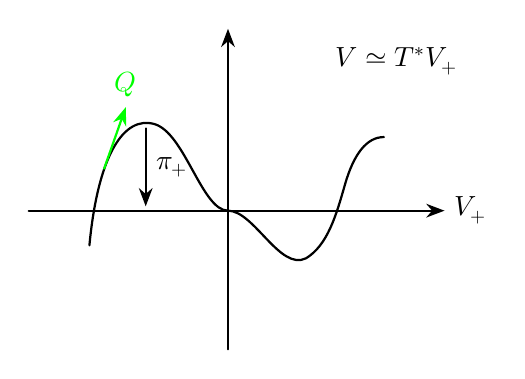
\begin{tikzpicture}[x=0.55cm,y=0.55cm,>=Stealth,line cap=round,line join=round]
  % axes
  \draw[thick,->] (-4.6,0) -- (5.0,0) node[right] {$V_+$};
  \draw[thick,->] (0,-3.2) -- (0,4.2);

  % labels
  \node at (3.9,3.45) {$V \simeq T^* V_+$};

  % curve
  \draw[thick]
    (-3.2,-0.8)
    .. controls (-3.0,1.3) and (-2.4,2.2) .. (-1.7,2.0)
    .. controls (-1.0,1.8) and (-0.6,0.0) .. (0,0)
    .. controls (0.6,0.0) and (1.2,-1.4) .. (1.8,-1.1)
    .. controls (2.3,-0.8) and (2.5,-0.1) .. (2.7,0.6)
    .. controls (2.9,1.3) and (3.2,1.7) .. (3.6,1.7);
  \draw[thick,->, green] (-2.86,0.97) -- (-2.36,2.39) node[above] {$Q$};
  \draw[thick,->] (-1.9,1.9) -- (-1.9,0.1) node[midway,right] {$\pi_+$};
\end{tikzpicture}
\end{center}
\caption{\(Q\) tangent to \(\mc{L}\) and the map \(\pi_+\).}%
\label{fig:tangent-vector-field}
\end{figure}

We will now return to our original infinite-dimensional setting of the B-model on a Calabi-Yau manifold \(X\). The structure is a bit more complicated but is still similar. Recall that
\[ Q \colon \ms{S}_-(X) \to \ms{S}_+(X) \oplus \ms{S}_-(X). \]
Also recall that
\[ \omega(-,-) = \on{Tr}(-,-) \on{Res}_{t = 0} (- \cdot -). \]
The problem comes from the trace pairing, which causes the Poisson tensor \(\omega^{-1}\) to involve distributions as
\[ \omega^{-1} = \sum_{k \in \Z} \delta_{\Delta} t^k \otimes (-t)^{-k-1}, \]
where \(\delta_{\Delta}\) is a distributional element of \(\ms{PV}(X) \otimes \ms{PV}(X)\) and is the integral kernel for the identity operator
\[ 1 \colon \ms{PV}(X) \to \ms{PV}(X). \]
Note that this is fine classically but will presernt problems for quantizing the theory. We can still write down the BV kernel
\begin{align*}
    P &= (\pi_+ \otimes \pi_+) [(Q \otimes 1) \omega^{-1}] \\
    &= (\partial \otimes 1) \delta_{\Delta}
\end{align*}
because \(Q\) only fails to preserve \(\ms{S}_-(X)\) on \(t^{-1} \ms{PV}\) via the \(t \partial\) term. Given a local functional \(I\) on \(\ms{S}_+(X) = \ms{PV}(X) \ps{t}\) of the form \(I = I(\mu_k) = \int \cdots,\) its variation can be computed as
\begin{align*}
    \delta I = \sum_k \on{Tr} \ab(\delta \mu_k \fdv{I}{\mu_k}).
\end{align*}
We define the BV bracket for two local functionals \(I_1\) and \(I_2\) by
\[ \ab\{ I_1, I_2 \}_0 = \on{Tr} \ab(\fdv{I_1}{\mu_0}) \partial \ab(\fdv{I_2}{\mu_0}), \]
which produces another local functional. Copying the finite-dimensional case, we have the following theorem.

\begin{thm}[Costello-Li]
    The BCOV action \(I_0^X = \on{Tr}\ab<e^{\mu}>_0\) satisfies the \textit{classical master equation}
    \[ Q I_0^X + \frac{1}{2} \ab\{ I_0^X, I_0^X \}_0 = 0. \]
\end{thm}

\begin{rmk}
    The theorem is proved directly in the lecturer's PhD thesis, where he finds that the classical master equation is equivalent to the genus-zero topological recursion relations. 
\end{rmk}

\section{Quantum master equation}%
\label{sec:Quantum master equation}

Note that the map \(\pi_+ \circ \mc{P} \colon \ms{S}_+(X) \to \ms{S}_+(X)\) is a diffeomorphism. However, we gain the classical interaction \(I_0^X\) and the Maurer-Cartan equation with respect to \(\delta\) becomes
\[ Q \mu + \sum_{k \geq 2} \frac{1}{k!} \ell_k (\mu^{\otimes k}) = 0, \]
where \(\ell_2, \ell_3, \ldots\) emerge from the \(\ab\{ I_0^X, -\}\) term.

We will now return to our toy model \((V, Q, \omega)\) of a dg symplectic vector space. We also continue to assume the Poisson kernel \(\omega^{-1}\) and the isotropic splitting \(V = V_+ \oplus V_-\). \(Q\) preserves \(V_+\) but not \(V_-\), and we wrote down the tensor
\[ P = \pi_+ \otimes \pi_+ [(Q \otimes 1)\omega^{-1}] \in \Sym^2(V_+). \]
This produced a dGBV algebra
\[ (\mc{O}(V_+), Q, \partial_P, \ab\{-,-\}_P) \]

\begin{defn}
    We define the (formal) \textit{Weyl algebra} 
    \[ \mc{W}(V) \coloneqq \prod_{n \geq 0} (V^*)^{\otimes n} \ps{\hslash} \Bigm/ \sim, \]
    where \(\hslash\) is the formal (quantum) parameter and the relation \(\sim\) is generated by
    \[ [a,b] \coloneqq a \otimes b - (-1)^{\abs{a}\abs{b}} b \otimes a \sim \hslash \omega^{-1}(a \otimes b). \]
\end{defn}

Note that the classical limit
\[ \mc{W}(V) / \hslash \simeq \hat{\mc{O}}(V) \]
is the formal functions on \(V\). We denote the annihilator \(\on{Ann}(V_+) \subset V^*\) to be 
\[ \on{Ann}(V_+) = \ab\{ \varphi \in V^* \mid \varphi(V_+) = 0 \}. \]
Because the differential \(Q\) preserves \(V_+\), the induced differential \(Q \colon V^* \to V^*\) preserves \(\on{Ann}(V_+)\) as well.

\begin{prop}
    The annihilator \(\on{Ann}(V_+) \subset V^*\) is a subcomplex.
\end{prop}

\begin{defn}
    The (formal) \textit{Fock space} is defined by
    \[ \Fock(V_+) \coloneqq \mc{W}(V) / \mc{W}(V) \on{Ann}(V_+). \]
\end{defn}

\begin{rmk}
    We treat \(\on{Ann}(V_+)\) as annihilation operators.
\end{rmk}

Because \(Q\) is compatible with \(\omega\), we see that \((\mc{W}(V), Q)\) defines a cochain complex with subcomplex \(\mc{W}(V) \on{Ann}(V_+) \subset \mc{W}(V)\). This induces a differential
\[ Q \colon \Fock(V_+) \to \Fock(V_+). \]
The splitting \(V = V_+ \oplus V_- \simeq T^* V_+\) induces a natural embedding \(V_+^* \subset V^*\) given by extension by zero on \(V_-\). Let
\[ \hat{\mc{O}}(V_+) \coloneqq \prod_{n \geq 0} \Sym^n (V_+^*) \]
be the formal functions on \(V_+\). This induces
\begin{equation*}
\begin{tikzcd}
    \hat{\mc{O}}(V_+)\ps{\hslash} \ar[hookrightarrow]{r} \ar{dr}{\Phi}[swap]{\simeq} & \mc{W}(v) \ar{d} \\
    & \Fock(V_+)
\end{tikzcd}
\end{equation*}
and realizes \(\hat{\mc{O}}(V_+) \ps{\hslash}\) as creation operators (which for physicists look like expressions of the form \(\cdots a^{\dagger} \ket{0}\)). Under this isomorphism, there is a differential \(\hat{Q}\) on \(\hat{\mc{O}}(V_+) \ps{\hslash}\), namely the unique one making the diagram
\begin{equation*}
\begin{tikzcd}
    \hat{\mc{O}}(V_+) \ps{\hslash} \ar{r}{\Phi} \ar{d}{\hat{Q}} & \Fock(V_+) \ar{d}{Q} \\
    \hat{\mc{O}}(V_+) \ps{\hslash} \ar{r}{\Phi} & \Fock(V_+)
\end{tikzcd}
\end{equation*}
commute. However, this is not the same as the one induced from \(Q \colon V_+ \to V_+\) (which extends to \(Q \colon \hat{O}(V_+) \to \hat{\mc{O}}(V_+)\)).

\begin{prop}
    The difference between \(\hat{Q}\) and \(Q\) is precisely the failure of \(Q\) to preserve the splitting, namely
    \[ \hat{Q} = Q + \hslash \partial_P. \]
\end{prop}

\begin{proof}
    This is standard quantization of quadratic Hamiltonians and is left as an exercise.
\end{proof}

\begin{defn}
    A formal function
    \[ F = \sum_{g \geq 0} F_g \hslash^g \in \hat{\mc{O}}(V_+) \ps{\hslash} \]
    satisfies the \textit{quantum BV master equation (QME)} if
    \[ (Q + \hslash \partial_P) e^{F/\hslash} = 0. \]
    Equivalently, we can rewrite this as
    \[ (Q + \hslash \partial_P) F + \frac{1}{2} \ab\{ F, F \}_P = 0. \]
    Note that in the classical limit \(\hslash \to 0\), we recover the classical master equation
    \[ Q F_0 + \frac{1}{2} \ab\{ F_0, F_0 \}_P = 0. \]
\end{defn}

We now discuss what is going on in a physical sense. Consider the state
\[ \ket{F} \coloneqq \Phi \ab(e^{F/\hslash}) = e^{F/\hslash} \ket{0}. \]
Then the quantum master equation is equivalent to the statement that \(Q \ket{F} = 0\), which in physics is called the \textit{quantum gauge consistency}. Passing to \(Q\)-cohomology (what physicists call \textit{physical states}), we pass to
\[ [\ket{F}] \in H^{\bullet}(\Fock(V_+), Q), \]
which usually an element of a finite-dimensional space. If we let \(\mc{H} = H^{\bullet}(V, Q)\) and \(\mc{H}_+ = H^{\bullet}(V_+, Q)\), then we have a symplectic vector space \((\mc{H}, \omega)\) with \(\mc{H}_+ \subset \mc{H}\) as an isotropic subspace. If we choose a polarization \(\mc{H} = \mc{H}_+ \oplus \mc{L}\), the surjection \(\mc{W}(V) \twoheadrightarrow \Fock(V_+)\) reduces to a surjection
\[ \on{\mc{W}eyl}(\mc{H}) \twoheadrightarrow \Fock(\mc{H}_+), \]
and the target is once again isomorphic to \(\hat{\mc{O}}(\mc{H}_+) \ps{\hslash}\) because the polarization gives an embedding \(\mc{H}_+^*\subset\mc{H}^*\). Because \(Q \ket{F} = 0\), we obtain a state
\[ [\ket{F}] \in \Fock(\mc{H}_+) \cong H^{\bullet}(\Fock(V_+), Q). \]
The choice of splitting gives us a formal function
\[ F^{\mc{L}} = \sum_{g \geq 0} F_g^{\mc{L}} \hslash^g \in \hat{\mc{O}}(\mc{H}_+) \ps{\hslash}. \]
Unfortunately, this is extremely hard to compute.

\begin{warn}
    If we try to redo everything in the actual B-model, the ``quantum master equation''
    \[ (Q + \hslash \partial_P) e^{F/\hslash} = 0 \]
    is ill-defined because \(P\) is singular. This will require choosing a K\"ahler metric, doing renormalization, and defining everything in a homotopical way.
\end{warn}




\section{Homotopic renormalization}%
\label{sec:Homotopic renormalization}

In quantum theory, we will replace \((V_+, Q)\) by \(\mc{E}, Q\), where \(\mc{E}\) is the space of fields. Usually, we will take
\[ \mc{E} = \Gamma(X, E^{\bullet}) \]
to be the global (smooth) sections of some graded vector bundle and 
\[ Q \colon \mc{E} \to \mc{E} \]
to be an elliptic operator (for example \(\dbar\) or \(\partial\)). This data \((\mc{E}, Q)\) will be called an \textit{elliptic complex}. The (shifted) symplectic space will be replaced by a (shifted) Poisson kernel \(P\), which is a distributional section of \(\Sym^2(\mc{E})\) which is usually supported on the diagonal of \(X \times X\) (here, note that \(P\) comes from the inverse of integration, which involves delta functions).

We will now follow the toy model until we reach an obstruction. The first modification we need to make is to force \(\mc{E}^* = \Hom_{\ms{cont}}(\mc{E}, \C)\) to be the continuous dual (these are essentially distributions on \(X\)). The next modification we need is to consider that \(\mc{E}^*\) is a nuclear space, so when we write \(\mc{E}^* \otimes \mc{E}^*\), we mean the completed tensor product, which we think of as distributions on \(X \times X\). This allows us to define
\[ \Sym^n (\mc{E}^*) \subset (\mc{E}^*)^{\otimes n}. \]
We may now discuss functions on \(\mc{E}\) as
\[ \mc{O}(\mc{E}) = \prod_{n \geq 0} \Sym^n (\mc{E}^*). \]
Our next goal is to define the BV operator, which in the toy model was \[\partial_P \colon \Sym^n(V_+^*) \to \Sym^{n-2}(V_+^*).\] We would like to define
\[ \partial_P \colon \Sym^n(\mc{E}^*) \to \Sym^{n-2}(\mc{E}^*), \]
but this is not well-defined because we cannot pair two distributions, which in QFT is known as the \textit{ultraviolet problem} and arises in any infinite-dimensional model.

We will resolve this problem by using Costello's \textit{homotopic renormalization theory}. We will change notation and replace \(P\) by \(K_0 \in \ms{Dist}(\Sym^2(\mc{E}))\), which is the (shifted) Poisson kernel. This is \(Q\)-closed, namely that
\[ Q(K_0) = (Q \otimes 1 + 1 \otimes Q) K_0 = 0. \]
The key observations are
\begin{enumerate}
    \item \(K_0\) is a \(Q\)-closed distribution;
    \item Elliptic regularity means that
    \[ H^{\bullet}(\ms{Smooth}, Q) \cong H^{\bullet}(\ms{Distributions}, Q) \]
    and therefore we can write
    \[ K_0 = K_r + Q(P_r), \]
    where \(K_r\) is a smooth kernel and \(P_r\) is a distribution known as the \textit{parametrix}.
\end{enumerate}
We will call \(K_r\) the \textit{renormalized BV kernel} with respect to the parametrix \(P_r\). Now, we can define
\[ \partial_{K_r} \colon \Sym^n(\mc{E}^*) \to \Sym^{n-2}(\mc{E}^*) \]
by contracting with the smooth kernel \(K_r\). This is now well-defined and gives us a \textit{renormalized BV operator}
\[ \partial_{K_r} \colon \mc{O}(\mc{E}) \to \mc{O}(\mc{E}). \]
(Note that working with formal power series means we are working perturbatively, and the non-perturbative theory is much more complicated). Because \(K_r\) is \(Q\)-closed, we see that
\[ [Q, \partial_{K_r}] = 0. \]

\begin{defn}
    The data \((\mc{O}(\mc{E}), Q, \partial_{K_r})\) defines a dGBV algebra called the \textit{renormalized dGBV} with respect to the parametrix \(P_r\).
\end{defn}

\begin{quest}
    How do we resolve the possible dependence on the choice of parametrix \(P_r\)?
\end{quest}

Let \(P_{r_1}\) and \(P_{r_2}\) be two parametrices such that
\[ K_0 = K_{r_1} + Q(P_{r_1}) = K_{r_2} + Q(P_{r_2}). \]
Then we see that \(P_{r_1}^{r_2} \coloneqq P_{r_2} - P_{r_1}\) is smooth inside \(\Sym^2(\mc{E})\).

\begin{defn}
    Define the operator
    \[ \partial_{P_{r_1}^{r_2}} \colon \mc{O}(\mc{E}) \to \mc{O}(\mc{E}) \]
    by contracting with the smooth kernel \(P_{r_1}^{r_2}\). 
\end{defn}

\begin{prop}
    The following diagram commutes:
    \begin{equation*}
    \begin{tikzcd}
        \mc{O}(\mc{E})\ps{\hslash} \ar{r}{Q + \hslash \partial_{K_{r_1}}} \ar{d}[swap]{\exp\ab(\hslash \partial_{P_{r_1}^{r_2}})} & \mc{O}(\mc{E})\ps{\hslash} \ar{d}{\exp\ab(\hslash \partial_{P_{r_1}^{r_2}})} \\
        \mc{O}(\mc{E})\ps{\hslash} \ar{r}{Q + \hslash \partial_{K_{r_2}}} & \mc{O}(\mc{E})\ps{\hslash}.
    \end{tikzcd}
    \end{equation*}
\end{prop}

\begin{proof}
    Note that \(K_{r_1} - K_{r_2} = Q(P_{r_1}^{r_2})\). This implies that
    \[ \ab[Q, \partial_{P_{r_1}^{r_2}}] = \partial_{K_{r_1}} - \partial_{K_{r_2}}. \]
    This implies that
    \begin{align*}
        e^{\hslash \partial_{P_{r_1}^{r_2}}} Q e^{-\hslash \partial_{P_{r_1}^{r_2}}} &= Q + \hslash \ab[\partial_{P_{r_1}^{r_2}}, Q] \\
        &= Q + \hslash \partial_{K_{r_2}} - \hslash \partial_{K_{r_1}}. \qedhere
    \end{align*}
\end{proof}

\begin{defn}
    Define
    \[ \mc{O}^+(\mc{E}) \ps{\hslash} \coloneqq \Sym^{\geq 3}(\mc{E}^*) \oplus \hslash \mc{O}(\mc{E}) \ps{\hslash}. \]
    Note that in physics this is called \textit{interaction theory}. We define the \textit{homotopic renormalization group flow}
    \[ W(P_{r_1}^{r_2}, I) \colon \mc{O}^+(\mc{E}) \ps{\hslash} \to \mc{O}^+(\mc{E}) \ps{\hslash} \]
    by the formula
    \[ W(P_{r_1}^{r_2}, I) \coloneqq \hslash \log \ab( e^{\hslash \partial_{P_{r_1}^{r_2}}} e^{I/\hslash}). \]
\end{defn}

The real content is that
\[ e^{W(P_{r_1}^{r_2}, I)/\hslash} = e^{\hslash \partial_{P_{r_1}^{r_2}}} e^{I/\hslash}. \]
This tells us that 
\[ W(P_{r_1}^{r_2}, I) \coloneqq \sum_{\Gamma \text{ connected}} W_{\Gamma}(P_{r_1}^{r_2}, I) \]
is a sum over connected Feynman diagrams, where contributions are as in~\Cref{fig:feynman-diagram}. The physicists would call \(I\) the \textit{vertex} and \(P_{r_1}^{r_2}\) the \textit{propagator}. 

\begin{figure}[htpb]
\begin{center}
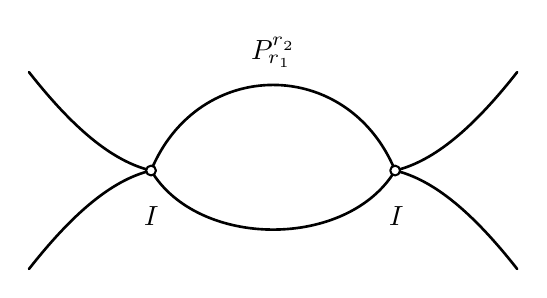
\begin{tikzpicture}[
  x=1cm,y=1cm,
  line cap=round,line join=round,
  curve/.style={line width=0.95pt},
  crossing/.style={circle,draw,fill=white,inner sep=1.25pt,line width=0.75pt},
  >=Latex
]
  % Key points
  \coordinate (L) at (-1.55,0);
  \coordinate (R) at ( 1.55,0);

  % Upper curve
  \draw[curve]
    (-3.10,-1.25)
    .. controls (-2.55,-0.55) and (-2.05,-0.12) .. (L)
    .. controls (-0.95,1.45) and (0.95,1.45) .. (R)
    .. controls (2.05,-0.12) and (2.55,-0.55) .. (3.10,-1.25);

  % Lower curve
  \draw[curve]
    (-3.10,1.25)
    .. controls (-2.55,0.55) and (-2.05,0.12) .. (L)
    .. controls (-0.95,-1.00) and (0.95,-1.00) .. (R)
    .. controls (2.05,0.12) and (2.55,0.55) .. (3.10,1.25);

  % Intersection markers + labels
  \node[crossing] at (L) {};
  \node[crossing] at (R) {};
  \node at ($(L)+(0,-0.58)$) {$I$};
  \node at ($(R)+(0,-0.58)$) {$I$};

  % Top annotation
  \node at (0,1.5) {$P^{r_2}_{r_1}$};
\end{tikzpicture}
\end{center}
\caption{Feynman diagram representation of the homotopic renormalization group flow.}%
\label{fig:feynman-diagram}
\end{figure}

\begin{defn}
    A solution of the \textit{effective quantum master equation} is an assignment \(I[r] \in \mc{O}^+(\mc{E})\ps{\hslash}\) for each parametrix \(P_r\) satisfying
    \begin{enumerate}
        \item The \textit{renormalized quantum master equation (RQME)}
        \[ (Q + \hslash \partial_{K_r}) e^{I[r]/\hslash} = 0; \]
        \item For any two parametrices \(P_{r_1}\) and \(P_{r_2}\), we have
        \[ I[r_2] = W(P_{r_1}^{r_2}, I[r_1]). \]
    \end{enumerate}
\end{defn}
Because of the chain homotopy
\[ e^{\hslash \partial_{P_{r_1}^{r_2}}} (Q + \hslash \partial_{K_{r_1}}) = (Q + \hslash \partial_{K_{r_2}}) e^{\hslash \partial_{P_{r_1}^{r_2}}}, \]
we see that the two conditions are compatible. The picture is as in~\Cref{fig:homotopic-renormalization}, where the two points \(r_1\) and \(r_2\) represent two different choices of parametrix and the arrow represents the homotopic renormalization group flow. The central dot represents the original singular kernel \(K_0\), which is homotopic to both \(K_{r_1}\) and \(K_{r_2}\) via the parametrices \(P_{r_1}\) and \(P_{r_2}\).

\begin{figure}[htpb]
\begin{center}
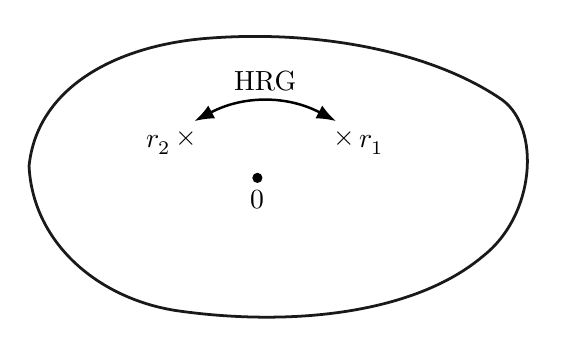
\begin{tikzpicture}[
  x=1cm,y=1cm,
  line cap=round,line join=round,
  >=Latex
]
  \tikzset{
    boundary/.style={line width=1pt, draw=black!90},
    flow/.style={line width=0.9pt,<->},
    pt/.style={circle,fill=black,inner sep=1.3pt},
    ring/.style={circle,draw,line width=0.9pt,minimum size=5.5pt,inner sep=0pt}
  }

  % Outer region
  \draw[boundary]
    (-3.15,0.10)
    .. controls (-3.05,1.08) and (-2.08,1.62) .. (-0.92,1.72)
    .. controls (0.52,1.84) and (1.98,1.55) .. (2.86,0.94)
    .. controls (3.35,0.58) and (3.28,-0.52) .. (2.62,-1.04)
    .. controls (1.75,-1.78) and (0.18,-1.94) .. (-1.25,-1.74)
    .. controls (-2.24,-1.60) and (-3.10,-0.90) .. (-3.15,0.10)
    -- cycle;

  % Marked points/labels
  \coordinate (A) at (-1.15, 0.45);
  \coordinate (B) at ( 0.85, 0.45);
  \node at (A) {$\times$};
  \node at (B) {$\times$};

  \node at ($(B)+(0.35,-0.08)$) {$r_1$};
  \node at ($(A)+(-0.35,-0.08)$) {$r_2$};

  % Curved arrow with label
  \draw[flow] ($(A)+(0.10,0.22)$) to[bend left=28] node[above] {HRG} ($(B)+(-0.10,0.22)$);

  % Central dot and small circle
  \coordinate (C) at (-0.25,-0.05);
  \node[pt]   at (C) {};
  \node at ($(C)+(0,-0.28)$) {$0$};
\end{tikzpicture}
\end{center}
\caption{Homotopic renormalization group flow.}%
\label{fig:homotopic-renormalization}
\end{figure}

\section{Quantum BCOV theory}%
\label{sec:Quantum BCOV theory}

We are finally ready to discuss the quantum B-model. Recall that our space of fields is
\[ \mc{E} = \ms{S}_+(X) = \ms{PV}(X) \ps{t}[2] \]
with \(Q = \dbar + t \partial\), which had the (shifted) Poisson kernel
\[ K_0 = (\partial \otimes 1) \delta_{\Delta} \in \ms{Dist}(\ms{PV}(X) \otimes \ms{PV}(X)). \]
Because this kernel is singular, we will need to run the homotopic renormalization group flow. First, choose a K\"ahler metric \(g\) on \(X\). This gives us
\[ \dbar^* \colon \ms{PV}^{i,j}(X) \to \ms{PV}^{i,j-1}(X) \]
which is the adjoint of \(\dbar\). We can then write down the Laplacian and then the \textit{heat kernel}
\[ h_r^g \in \ms{PV}(X) \otimes \ms{PV}(X) \]
for any \(r > 0\), which represents
\[ \ab(e^{-r [\dbar, \dbar^*]}) (x_1) = \on{Tr}_{x_2} h_r^g (x_1, x_2) \alpha(x_2) \]
for any \(\alpha \in \ms{PV}(X)\). Now let
\[ K_r = (\partial \otimes 1) h_r^g \xrightarrow{r \to 0} K_0 \]
(this limit holds because the heat kernel converges to the delta function). Also, note that because of the grading,
\[ [\dbar, \dbar^*] = \dbar \dbar^* + \dbar^* \dbar \]
is the usual Laplacian. Now the parametrix is given by
\[ P_r = \int_0^r (\dbar^* \partial \otimes 1) h_u^g \d{u}. \]

\begin{prop}
    We have \(K_0 = K_r + Q(P_r)\).
\end{prop}

\begin{proof}
    This is the integral kernel representation of the operator equation
    \[ \partial = \partial e^{-r[\dbar, \dbar^*]} + \ab[Q, \int_0^r \dbar^* \partial e^{-u [\dbar, \dbar^*]} \d{u}]. \]
    Because \(Q = \dbar + t \partial\) and the K\"ahler condition implies that
    \[ [\dbar, \partial] = [\dbar^*, \partial] = 0, \]
    we see that
    \begin{align*}
        \ab[Q, \int_0^r \dbar^* \partial e^{-u [\dbar, \dbar^*]} \d{u}] &= \int_0^r [\dbar, \dbar^*] \partial e^{-u [\dbar, \dbar^*]} \d{u} \\
        &= \partial - \partial e^{-r [\dbar, \dbar^*]} \qedhere
    \end{align*}
\end{proof}

\begin{defn}
    Given \(0 < \ep < L\), define the \textit{effective propagator}
    \[ P_{\ep}^L = \int_{\ep}^L (\dbar^* \partial \otimes 1) h_u^g \d{u} \in \Sym^2 (\ms{PV}(X)) \subset \Sym^2(\mc{E}). \]
    This is the homotopy from \(K_{\ep}\) to \(K_L\).
\end{defn}

\begin{defn}[Costello-Li]
    A \textit{perturbative quantization} of BCOV theory on \(X\) is a family of functionals (or distributions)
    \[ F[L] = \sum_{g =0}^{\infty} \hslash^g F_g[L] \in \mc{O}^+(\ms{S}_+(X)) \ps{\hslash} \]
    for each \(L > 0\) such that
    \begin{enumerate}
        \item They respect the homotopic renormalization group flow, namely
        \[ F[L] = W(P_{\ep}^L, F[\ep]) \iff e^{F[L]/\hslash} = e^{\hslash \partial_{P_{\ep}^L}} e^{F[\ep]/\hslash}; \]
        \item The renormalized quantum master equation
        \[ (Q + \hslash \Delta_L) e^{F[L]/\hslash} = 0, \]
        where \(\Delta_L = \partial_{K_L}\), holds;
        \item The \textit{locality axiom} that \(F[L]\) has a small \(L\) asymptotic expansion by local functionals as \(L \to 0\);
        \item The classical limit
        \[ \lim_{L \to 0} F_0[L] = I_0^X, \]
        recovers the classical BCOV action;
        \item The degree axiom and Hodge weight axiom hold (this is analogous to Gromov-Witten theory) such that \(F_g^L\) has Hodge weight \((3-\dim X)(g-1)\), where \(t^m \ms{PV}^{k, \bullet}\) has Hodge weight \(k+m-1\).
    \end{enumerate}
\end{defn}

\begin{rmk}
    This quantization is not necessarily unique.
\end{rmk}

Given a quantization \(\ab\{ F[L]\}_L \), we consider the \textit{IR limit} \(K \to +\infty\). In this limit, we have
\[ K_L = (\partial \otimes 1) e^{-L [\dbar, \dbar^*]} \xrightarrow{L \to +\infty} (\partial \otimes 1) (\ms{Harmonics}) = 0, \]
and therefore the quantum master equation becomes
\[ Q e^{F[\infty]/\hslash} = 0. \]
This implies that \(Q F[\infty] = 0\), so it represents some cohomology class
\[ [F[\infty]]_Q \in H^{\bullet}(\mc{O}(\ms{S}_+(X)\ps{\hslash}), Q) \simeq \mc{O}(H^{\bullet}(\ms{S}_+(X), Q)) \ps{\hslash}. \]
A choice of K\"ahler metric \(g\) gives a splitting of the Hodge filtration, which gives an isomorphism
\[ H^{\bullet}(\ms{S}_+(X), Q) \simeq H^{\bullet}(X, \wedge^{\bullet} T_X) \ps{t}. \]
This now gives quantum B-model invariants \(F_{g,n,X}^{\mc{L}}\), which by the mirror conjecture should be related to the Gromov-Witten invariants \(\ab<->_{g,n,\check{X}}^{\ms{GW}}\) on the mirror \(\check{X}\).

Calculations are very hard, but we can do them using UV finiteness and locality. In practice, constructing a quantization is very complicated, but the program usually goes as follows.
\begin{enumerate}
    \item Start with a local functional \(I \in \mc{O}_{\ms{loc}}^{\dagger}(\mc{E})\ps{\hslash}\) (the classical interaction).
    \item Find an \(\ep\)-dependent local functional
    \[ I^{\ms{CT}}(\ep) \in \hslash \mc{O}_{\ms{loc}}(\mc{E})\ps{\hslash} \]
    such that the limit
    \[ e^{I[L]/\hslash} \coloneqq \lim_{\ep \to 0} e^{\hslash \partial_{P_{\ep}^L}} e^{(I + I^{\ms{CT}}(\ep))/\hslash} \]
    exists. If we can find the counterterms, the family \(\ab\{I[L]\}\) automatically satisfies the homotopic RG flow. However, it does not necessarily satisfy the quantum master equation.
    \item Find further corrections to solve the quantum master equation. This step may be obstructed, and the obstruction is known in physics as the \textit{gauge anomaly}.
\end{enumerate}

\begin{defn}
    We say the theory is \textit{UV finite} if the limit
    \[ I[L] \coloneqq \lim_{\ep \to 0} e^{\hslash \partial_{P_{\ep}^L}} e^{I/\hslash} \]
    exists for the class of local functionals \(I\) in question without the need for counterterms.
\end{defn}

Now assume that the theory is UV finite (all chiral theories like BCOV theory, holomorphic Chern-Simons, etc are in fact UV finite). Unfortunately, the equation
\[ \hslash \Delta I + Q I + \frac{1}{2} \ab\{ I, I \} = 0 \]
is ill-defined at \(L = 0\), so we regularize to an equation of the form
\[ \hslash \Delta_L I[L] + Q I[L] + \frac{1}{2} \ab\{ I[L], I[L] \}_L = 0. \]
If the theory is UV finite, we can take the \(L \to 0\) limit to obtain something like
\[ Q I + \frac{1}{2} \ab\{ I, I\} + \ell_3(I,I,I) + \cdots = 0, \]
where the \(\ell_k\) can be viewed as higher brackets for local functionals and come from resolving the ill-defined term \(\hslash \Delta I\). We will refer to this as the \textit{renormalized local quantum master equation}. Unfortunately, what the \(\ell_k\) are is not known in general.

\begin{exer}
    Do this for holomorphic Chern-Simons theory.
\end{exer}

There is one case where the higher brackets are known explicitly.

\begin{thm}[Li]
    2D chiral theories are UV finite and the renormalized local quantum master equation is equivalent to the Maurer-Cartan equation in chiral vertex operator algebras. 
\end{thm}

The renormalization behaves as in~\Cref{fig:renormalization}, and a reference is the paper~\href{https://doi.org/10.4310/jdg/1683307007}{Vertex algebras and quantum master equation} by the lecturer. From this, we can obtain an explicit canonical solution for the quantum B-model on elliptic curves and establish the quantum mirror conjecture.

\begin{figure}[htpb]
\begin{center}
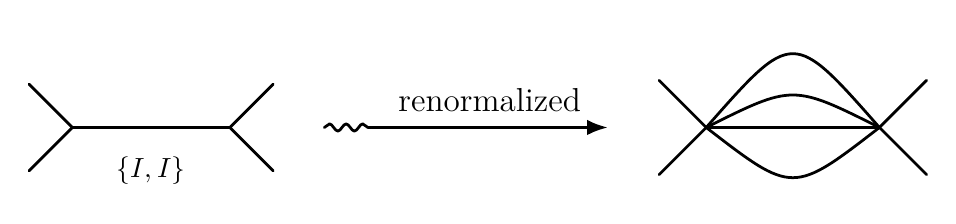
\begin{tikzpicture}[
  line cap=round,
  line join=round,
  >=Latex,
  feyn/.style={draw=black,line width=1pt}
]

% Left Feynman diagram
\coordinate (L1) at (-6,0);
\coordinate (L2) at (-4,0);
\draw[feyn] (L1) -- (L2);
\draw[feyn] (L1) -- ++(-0.55, 0.55);
\draw[feyn] (L1) -- ++(-0.55,-0.55);
\draw[feyn] (L2) -- ++( 0.55, 0.55);
\draw[feyn] (L2) -- ++( 0.55,-0.55);
\node[below=7pt] at (-5,0) {$\{I,I\}$};

% Middle "renormalized" arrow
\draw[feyn,decorate,decoration={snake,amplitude=1.3pt,segment length=6pt}] (-2.8,0) -- (-2.2,0);
\draw[feyn,->] (-2.2,0) -- (0.8,0) node[midway,above=2pt] {\large renormalized};

% Right Feynman diagram
\coordinate (R1) at (2.05,0);
\coordinate (R2) at (4.25,0);
\draw[feyn] (R1) -- (R2); % middle edge
\draw[feyn] (R1) .. controls (3.15, 1.25) .. (R2); % top loop
\draw[feyn] (R1) .. controls (3.15, 0.55) .. (R2); % inner top loop
\draw[feyn] (R1) .. controls (3.15,-0.85) .. (R2); % bottom loop
\draw[feyn] (R1) -- ++(-0.60, 0.60);
\draw[feyn] (R1) -- ++(-0.60,-0.60);
\draw[feyn] (R2) -- ++( 0.60, 0.60);
\draw[feyn] (R2) -- ++( 0.60,-0.60);

\end{tikzpicture}
\end{center}
\caption{Renormalization of 2D chiral theories}%
\label{fig:renormalization}
\end{figure}



\begin{thm}[Wang-Yan]
    Chiral theories of any dimension are UV finite (which implies that BCOV theory and holomorphic Chern-Simons theory are UV finite).
\end{thm}

The result of Wang-Yan implies that quantum BCOV theory has a local expression.

\begin{rmk}
    Gui calculated the higher chiral operator product expansions.
\end{rmk}



\section{Landau-Ginzburg B-model}%
\label{sec:Landau-Ginzburg B-model}

There are many ways to describe the Landau-Ginzburg B-model (for example via the category of matrix factorizations), but we will take the approach of string field theory. We will consider the Landau-Ginzburg B-model associated to the data \((X, \Omega, f)\), where
\begin{enumerate}
    \item \(X\) is a non-compact complex manifold;
    \item \(\Omega\) is a holomorphic volume form on \(X\);
    \item \(f\) is a holomorphic function\footnote{This forces us to work with non-compact manifolds.} (called the \textit{superpotential}) on \(X\) with compact critical locus (which we call \(\on{Crit}(f)\)).
\end{enumerate}

We will consider polyvector fields \(\ms{PV}(X) = \Omega^{0, \bullet}(X, \Lambda^{\bullet} T_X)\) and the compactly supported polyvector fields \(\ms{PV}_c(X) \subset \ms{PV}(X)\). We will twist the Dolbeault operator and write
\[ \dbar_f \coloneqq \dbar + \ab\{f, -\} = \dbar + \d{f} \lrcorner. \]
We will still refer to the divergence operator with respect to \(\Omega\) as \(\partial\). Then we can consider the dGBV algebras
\[ (\ms{PV}_c(X), \dbar_f, \partial) \subset (\ms{PV}(X), \dbar_f, \partial). \]

\begin{lem}
    The inclusion \((\ms{PV}_c(X), \dbar_f) \subset (\ms{PV}(X), \dbar_f)\) is a quasi-isomorphism.
\end{lem}

\begin{proof}
    The operation \(\ab\{f, -\}\) becomes the Koszul complex, which is exact outside of (a small neighborhood of) the critical locus \(\Crit(f)\).
\end{proof}

To apply the Barannikov-Kontsevich construction to obtain a Frobenius manifold on the cohomology \(H^{\bullet}(\ms{PV}, \dbar_f)\) , a number of things are required:
\begin{enumerate}
    \item Hodge-to-de Rham degeneration at the \(E_1\) page for the \(t\)-adic filtration on \(\ms{PV}(X) \ps{t}, \dbar_f + t \partial\) (or the compactly supported version), where unfortunately both are bad. If this exists, then this is smooth formal in the sense of Barannikov-Kontsevich and therefore has a univeral period map (which would give us a \(J\)-function allow us to write down the Frobenius structure);
    \item A trace pairing \(\on{Tr}(-,-)\) on polyvector fields which is compatible with \(\dbar_f\) and \(\partial\), which is required to write down a formula like
    \[ \omega = \on{Tr}(-,-) \on{Res}_{t = 0}, \]
    which of course works better for compactly supported polyvector fields;
    \item A compatible splitting
    \[ H^{\bullet}(\ms{PV}_c(X), \dbar_f) \to H^{\bullet}(\ms{PV}_c(X) \ps{t}, \dbar_f + t \partial) \]
    which is compatible with the trace pairing (and the higher residue pairing). This is usually referred to as a \textit{good basis}.
\end{enumerate}

\begin{rmk}
    When \(f\) has isolated critical points, the cohomology 
    \[ H^{\bullet}(\ms{PV}(X), \dbar_f) = \on{Jac}(f) = \mc{O}(\Crit(f)) \]
    and the Hodge-to-de Rham degeneration holds automatically.
\end{rmk}

To define the trace pairing, it is of course better to use \(\ms{PV}_c(X)\).

\begin{defn}
    Define the \textit{trace pairing}
    \[ \on{Tr} \colon \ms{PV}_c(X) \to \C \qquad \mu \mapsto \int_X (\mu \lrcorner \Omega) \wedge \Omega. \]
\end{defn}

\begin{prop}
    We have the formulae
    \begin{align*}
        \on{Tr}(\dbar_f \alpha \beta) &= -(-1^{\abs{\alpha}}) \on{Tr}(\alpha \dbar_f \beta), \\
        \on{Tr}(\partial \alpha \beta) &= (-1^{\abs{\alpha}}) \on{Tr}(\alpha \partial \beta).
    \end{align*}
\end{prop}

\begin{cor}
    The trace pairing defines a pairing on cohomology given by
    \[ \on{Tr} \colon H^{\bullet}(\ms{PV}_c(X), \dbar_f) \otimes H^{\bullet}(\ms{PV}_c(X), \dbar_f) \to \C \]
    and the higher residue pairing
    \[ K_f \colon H^{\bullet}(\ms{PV}_c(X) \ps{t}, Q_f) \otimes H^{\bullet}(\ms{PV}_c(X) \ps{t}, Q_f) \to \C \ps{t} \] 
    given by the formula 
    \[ \alpha f(t) \otimes \beta g(t) \mapsto \on{Tr}(\alpha\beta) f(t) g(-t). \]
\end{cor}

\begin{rmk}
    Assume that \(f \colon \C^n \to \C\) has only an isolated critical point at the origin. Let \(\Omega = \d^n z\) be the standard volume form. Then we have
    \[ H^{\bullet}(\ms{PV}_c(X), \dbar_f) \simeq \on{Jac}(f) \cong \Omega^n_{\ms{hol}} / \d{f} \wedge \Omega^{n-1}_{\ms{hol}} \eqqcolon \Omega_f. \]
    Then the trace pairing
    \[ \on{Tr} \colon \Omega_f \otimes \Omega_f \to \C \]
    is precisely the residue pairing, where we see that
    \[ \on{Tr} (\alpha(z) \d^n z, \beta(z) \d^n z) = \on{Res}_{z = 0} \frac{\alpha \beta \d^n z}{\partial_1 f \cdots \partial_n f}. \]
    A reference is the \href{https://arxiv.org/pdf/1311.1659}{paper by Changzheng Li, the lecturer, and Kyoji Saito}. In particular, if we write
    \[ K_f (\alpha(z), \beta(z)) = K_0(\alpha, \beta) + K_1(\alpha, \beta) t + \cdots, \]
    then \(K_0\) is the residue as just described, and all of the \(K_{>0}\) are called \textit{higher residues}. Here, we should consider holomorphic functions as elements of \(H^{\bullet}(\ms{PV}(X) \ps{t}, Q_f)\). 
\end{rmk}

Regarding the Hodge-to-de Rham degeneration issue, we can look at the various models:
\begin{itemize}
    \item \(\ms{PV}(X)\) behaves well here, but is bad for the trace pairing;
    \item \(\ms{PV}_c(X)\) behaves well for the trace pairing, but is too small for the Hodge decomposition (for example harmonic functions are outside of this);
    \item If we consider \(L^2\) polyvector fields, this works well for both the trace pairing and the Hodge decomposition, but is ``bad'' for non-linear structures (like products).
\end{itemize}

To solve these problems, we will introduce yet another model, which was introduced by the lecturer and Wen and are called \textit{adapted polyvector fields}. It will sit as
\[ \ms{PV}_c(X) \subset \ms{PV}_{f, \infty}(X) \subset \ms{PV}(X) \]
and will have integration, the Hodge decomposition, and non-linear structures (products) all be well-behaved. It is given by
\[ \ms{PV}_{f, \infty}(X) = \ab\{ \mu \in L^2 (\ms{PV}(X)) \mid \abs{\nabla f}^j \nabla^j \mu \in L^2 \text{ for all } i, j \}. \]

\begin{defn}
    The data \((X, g, \Omega)\) (here \(g\) is a complete K\"ahler metric) is called a \textit{bounded Calabi-Yau geometry} if \((X, g)\) is a bounded geometry (namely a complete Riemannian manifold, all derivatives of curvature are bounded, and positive injectivity radius), and all covariant derivatives of \(\Omega\) and \(\Omega^{-1}\) are bounded.
\end{defn}

\begin{defn}
    Let \((X, g)\) be a bounded geometry. A holomorphic function \(f \colon X \to \C\) is \textit{strongly elliptic} if for all \(\ep > 0\) and \(k \geq 2\), then \(\ep \abs{\nabla f}^k - \abs{\nabla^k f} \to +\infty\) as \(z \to \infty\) approaches the boundary.
\end{defn}

\begin{exm}
    Here are some examples which fall into this setup:
    \begin{enumerate}
        \item Let \((X, \Omega_X) = (\C^n \d^n z)\) and \(g\) be the standard flat metric. Next, let \(f\) be a non-degenerate quasi-homogeneous polynomial. This is mirror to FJRW theory and the full mirror theorem holds by the work of Li-Li-Saito-Shen and He-Li-Shen-Webb.
        \item Let \((X, \Omega_X) = \ab((\C^{\times})^n, \frac{\d{z_1}}{z_1} \wedge \cdots \wedge \frac{\d{z_n}}{z_n})\), \(g\) be the standard metric, and \(f\) be a convenient non-degenerate Laurent polynomial (here the origin lies in the interior of the Newton polytope). This is mirror to toric varieties;
        \item Let \(X \to \C^n / G\) be a crepant resolution for \(G \subset \on{SU}(n)\) is a finite subgroup and \(g\) be an ALE metric. The superpotential is given by \(f \colon \C^n \to \C\) which is \(G\)-invariant. This is the orbifold Landau-Ginzburg B-model. Note here, that the superpotential lifts as
        \begin{equation*}
        \begin{tikzcd}
            X \ar{d} \ar[dashed]{dr}{\hat{f}} \\
            \C^n / G \ar{r}{f} & \C.
        \end{tikzcd}
        \end{equation*}
    \end{enumerate}
\end{exm}

\begin{thm}[Li-Wen]
    Let \((X, g, \Omega)\) be a bounded Calabi-Yau geometry and \(f \colon X \to \C\) be holomorphic and strongly elliptic with compact critical locus.
    \begin{enumerate}
        \item The data \((\ms{PV}_{f, \infty}(X), \dbar_f, \partial)\) forms a dGBV algebra with the trace pairing and Hodge-to-de Rham degeneration holds;
        \item The inclusions \((\ms{PV}_c(X), \dbar_f) \subset (\ms{PV}_{f, \infty}(X), \dbar_f) \subset (\ms{PV}(X), \dbar_f)\) are all quasi\-/isomorphisms. In particular, Hodge-to-de Rham degeneration holds for \((\ms{PV}(X), \dbar_f, \partial)\) as well.
        \item (Poincar\'e duality) The trace map induces
        \[ \on{Tr} \colon H^{\bullet}(\ms{PV}_{f, \infty}(X), \dbar_f) \otimes H^{\bullet}(\ms{PV}_{f, \infty}(X), \dbar_f) \to \C, \]
        this is non-degenerate, and \(K_f\) generalizes Saito's higher residue pairing.
    \end{enumerate}
\end{thm}

The upshot is that a Frobenius manifold structure can be constructed on the cohomology \(H^{\bullet}(\ms{PV}(X), \dbar_f)\).

\begin{rmk}
    There is an algebraic approach based on positive characteristic methods, including the work of Sabbah, Ogus-Vologodsky, Esnault-Sabbah-Yu, and Katzarkov-Kontsevich-Pantev.
\end{rmk}

\section{Open-closed B-model}%
\label{sec:Open-closed B-model}

So far, we have discussed the B-model closed string field. This leads to a generalized version of BCOV theory, which was developed by Costello and the lecturer. We will now discuss the open-closed B-model. As a reminder, Witten in 1992 gave two models of the open string field theory.
\begin{itemize}
    \item The A-model open string field is Chern-Simons theory with instanton corrections;
    \item The B-model open string field is holomorphic Chern-Simons theory.
\end{itemize}

Let \(X\) be a Calabi-Yau threefold and \(E\) be a holomorphic vector bundle on \(X\). The space of fields will be
\[ \mc{E} = \Omega^{0, \bullet}(X, \End(E))[1] \ni A \]
and the action (in the BV formalism) is given by
\[ \ms{HCS}[A] = \int_X \on{Tr} \ab(\frac{1}{2}A \wedge \dbar A + \frac{1}{6} A \wedge [A,A]) \wedge \Omega. \]
If we decompose
\[ A = A_0 + A_1 + A_2 + A_3, \]
where \(A_i \in \Omega^{0,i}(X, \End(E))\), then \(A_0\) is the ghost, \(A_1\) is the gauge (physical) field, \(A_2\) is the anti-field, and \(A_3\) is the anti-ghost. For the physical field \(A_1\), the equation of motion is
\[ \dbar A_1 + \frac{1}{2} [A_1, A_1] = 0, \]
which says that if we set \(\bar{\nabla} = \dbar + A_1\), then \(\bar{\nabla}^2 = 0\), meaning \(\bar{\nabla}\) defines a new holomorphic vector bundle structure on \(E\). This is what is meant when it is said that holomorphic Chern-Simons theory describes the moduli of holomorphic vector bundles.

The space \(\mc{E}\) is \((-1)\)-shifted symplectic with the symplectic form
\[ \omega(\alpha, \beta) = \int_X \on{Tr}(\alpha \wedge \beta) \wedge \Omega. \]
The shifted Poisson kernel is given by
\[ \omega^{-1} = \delta_{\Delta} \in \ms{Dist}(\mc{E} \otimes \mc{E}) \]
and defines a BV bracket \(\ab\{I_1, I_2\}_o\) for local functionals \(I_1, I_2\). Holomorphic Chern-Simons theory satisfies the classical master equation
\[ \ab\{ \ms{HCS}, \ms{HCS} \}_o = 0. \]
If we write \(\delta_{\ms{HCS}} = \ab\{ \ms{HCS}, -\}_o\) (the BRST transformation), then we obtain
\[ \delta_{\ms{HCS}} A = \dbar A + \frac{1}{2} [A, A], \]
and this implies that \(\delta_{\ms{HCS}}^2 = 0\). Equivalently, this says that \(\Omega^{0, \bullet}(X, \End(E))\) is a dg Lie algebra.

A bit more universally, embed \(E \hookrightarrow L^{\oplus N}\) as a subbundle for some sufficiently ample line bundle \(L\). This allows us to represent \(E\) by some idempotent matrix
\[ P \in \mf{gl}_N(C^{\infty}(X)) \]
by choosing a smooth splitting. Using this, we write \(E = P(L^{\oplus N})\), and then we can embed
\[ \Omega^{0, \bullet}(X, \End(E)) \hookrightarrow \Omega^{0, \bullet}(X, \mf{gl}_N). \]
Here, \(N\) must be very large, so we will consider the behavior as \(N \to \infty\). We will focus on
\[ \mc{E}_n = \Omega^{0, \bullet}(X) \otimes \mf{gl}_N [1] \subset \mc{E}_{n+1} \subset \cdots \]
and look for functionals on \(\mc{E}_N\) which have a stable expression when \(N \to \infty\). We will call these \textit{admissible functionals}.

\begin{exm}
    The functional
    \[ \int_X \on{Tr} A^3 \wedge \Omega \]
    is admissible.
\end{exm}

We will now study the large \(N\) limit from the perspective of large \(N\) duality. For \(A \in \mc{E}_N\), we can write
\[ \ms{HCS} = \int_X \on{Tr} \ab(\frac{1}{2} A \wedge \dbar A + \frac{1}{3} A^3) \wedge \Omega. \]
Unlike ordinary Chern-Simons theory (which only allows us to tune the coupling constant), holomorphic Chern-Simons has many degrees of freedom to deform. One deformation is to deform the Calabi-Yau structure, and in fact this gives all deformations. Consider a first order deformation 
\[ \ms{HCS} \to \ms{HCS} + J, \]
where \(J\) is an admissible local functional. The first-order classical master equation says that
\[ \delta_{\ms{HCS}} J = \ab\{\ms{HCS}, J\}_o = 0. \]
\(J\) is the local dual of Lie algebra homology
\[ H_{\bullet}^{\ms{Lie}}(\gl_N \Omega^{0, \bullet} \otimes \gl_N), \]
where the differential is \(\dbar\) and the Lie bracket is given by \([-,-]\). This looks hard to compute, but in fact there is a way to compute it.

\begin{thm}[Loday-Quillen-Tsygan]
    The large \(N\) limit of the Lie algebra homology is given by
    \[ \lim_{N \to +\infty} H_{\bullet}(\mf{gl}_N(R)) = \Sym(\ms{HC}_{\bullet-1}(R)). \]
    Here, \(\ms{HC}\) is called \textit{cyclic homology}.
\end{thm}

Applying this to our model, we obtain
\begin{align*}
    \ms{HC}_{\bullet}(\Omega^{0, \bullet}(X)) &\simeq (\Omega^{\bullet, \bullet}(X)[t^{-1}], \dbar + t \partial) \\
    &= (\Omega^{\bullet, \bullet}(X) \ls{t^{-1}} / t \Omega^{\bullet, \bullet}(X) \ps{t^{-1}}, \dbar + t \partial)
\end{align*}
by the Hochschild-Kostant-Rosenberg theorem (use \(\ms{HC}_{\bullet}(R) \sim (C_{\bullet}(R)[t^{-1}], b + tB)\)).
By the trace pairing, this is local dual to 
\[ (\ms{PV}(X) \ps{t}, Q = \dbar + t \partial). \]
Therefore, the BCOV field (topological gravity) is the single trace operator at \(N \to +\infty\) (this is also related to the AdS/CFT correspondence) in the \textit{gauge/gravity duality}.

\begin{exm}
    Suppose \(\mu \in \ms{PV}^{k, \bullet}(X)\). This gives a first-order deformation
    \[ J_{\mu} = \int_X \on{Tr} (\mu \lrcorner A \wedge \partial A \wedge \cdots \wedge \partial A) \wedge \Omega, \]
    which is in fact another way to express the HKR theorem.
\end{exm}

\begin{exm}
    If we include descendents to make \(\mu \in t^m \ms{PV}^{k, \bullet}(X)\), then (see~\Cref{fig:descendentdeformation})
    \[ J_{\mu} = \sum_{\ell_1 + \cdots + \ell_k = 2m} \int_X \on{Tr} (\mu \lrcorner A \wedge \partial A \wedge A^{\ell_1} \wedge \cdots \wedge A^{\ell_k}) \wedge \Omega. \]
    \begin{figure}[htpb]
    \begin{center}
    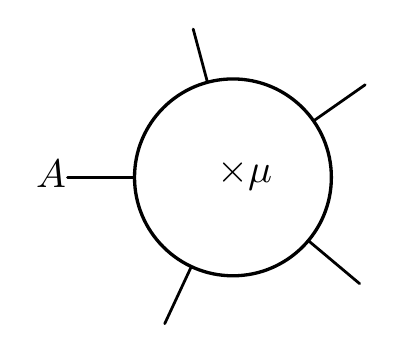
\begin{tikzpicture}[
  x=1cm,y=1cm,
  line cap=round,line join=round,
  edge/.style={line width=1pt},
  blob/.style={line width=1.2pt}
]
  % Main interaction blob
  \def\r{1.25}
  \draw[blob] (0,0) circle (\r);

  % External legs
  \foreach \ang/\len in {180/0.85,105/0.70,35/0.80,-40/0.85,-115/0.80}{
    \draw[edge]
      ({\r*cos(\ang)},{\r*sin(\ang)})
      -- ++({\len*cos(\ang)},{\len*sin(\ang)});
  }

  % Labels
  \node[font=\Large] at (-2.3,0.05) {$A$};
  \node[font=\Large] at (0.15,0.0) {$\times \mu$};
\end{tikzpicture}
    \end{center}
    \caption{$\mu$ at the bulk and \(A\) at the boundary.}%
    \label{fig:descendentdeformation}
    \end{figure}
A general formula for higher order deformations at the disk level is given by Calaque-Willwacher's cyclic extension of Kontsevich formality (see~\Cref{fig:higherorderdeformation}). This is called a \textit{Poisson \(\sigma\)-model} with formulae given by
\[ \int_{\ms{Conf}_{n,m}(D^2)} \cdots \]
\begin{figure}[htpb]
\begin{center}
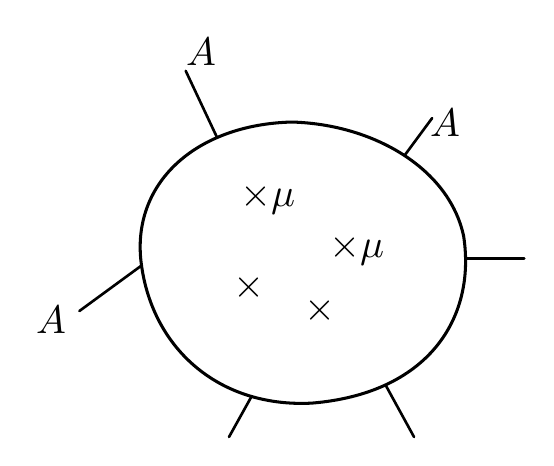
\begin{tikzpicture}[
  x=1cm,y=1cm,
  line cap=round,
  line join=round,
  blob/.style={draw=black,fill=white,line width=1.1pt},
  leg/.style={draw=black,line width=0.95pt}
]
  % External legs
  \draw[leg] (-0.95, 1.35) -- (-1.35, 2.20);
  \draw[leg] ( 1.30, 0.95) -- ( 1.78, 1.60);
  \draw[leg] ( 2.18,-0.18) -- ( 2.95,-0.18);
  \draw[leg] ( 1.15,-1.72) -- ( 1.55,-2.45);
  \draw[leg] (-0.45,-1.82) -- (-0.80,-2.45);
  \draw[leg] (-1.88,-0.25) -- (-2.70,-0.85);

  % Main blob
  \draw[blob]
    (0,1.55)
    .. controls (1.05,1.52) and (2.00,0.95) .. (2.18,0.10)
    .. controls (2.34,-0.95) and (1.72,-1.90) .. (0.25,-2.02)
    .. controls (-0.95,-2.08) and (-1.80,-1.30) .. (-1.92,-0.20)
    .. controls (-2.02,0.80) and (-1.20,1.52) .. (0,1.55)
    -- cycle;

  % Outside labels
  \node[font=\Large] at (-1.15, 2.45) {$A$};
  \node[font=\Large] at ( 1.95, 1.55) {$A$};
  \node[font=\Large] at (-3.05,-0.95) {$A$};

  % Interior markings
  \node[font=\Large] at (-0.30, 0.55) {$\times \mu$};
  \node[font=\Large] at ( 0.82,-0.10) {$\times \mu$};
  \node[font=\Large] at (-0.55,-0.55) {$\times$};
  \node[font=\Large] at ( 0.35,-0.85) {$\times$};
\end{tikzpicture}
\end{center}
\caption{Higher order deformation}%
\label{fig:higherorderdeformation}
\end{figure}
\end{exm}

We will now discuss the open-closed master equation. We are interested in distributions
\[ I_{g, h}[\mu, A] \]
where \(g\) is the genus and \(h\) is the number of boundary components. 

\begin{figure}[htpb]
\begin{center}
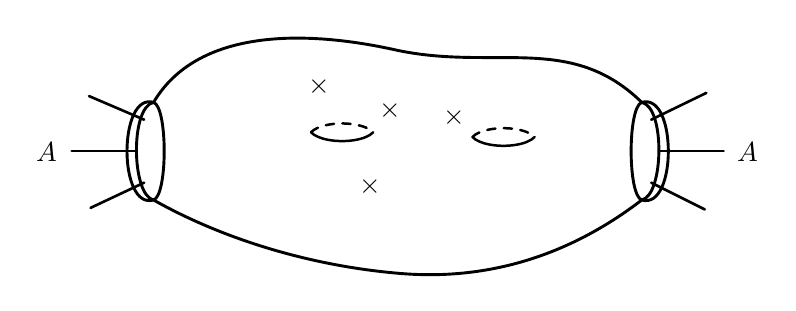
\begin{tikzpicture}[
  x=1cm,y=1cm,
  line cap=round,
  line join=round,
  surf/.style={draw=black,line width=1.05pt},
  hole/.style={draw=black,line width=0.9pt},
  holeback/.style={draw=black,line width=0.9pt,dashed},
  leg/.style={draw=black,line width=0.95pt}
]
  % Boundary components
  \coordinate (L) at (-3.10,0);
  \coordinate (R) at ( 3.10,0);
  \coordinate (Lt) at ($(L)+(0,0.62)$);
  \coordinate (Ll) at ($(L)+(-0.22,0)$);
  \coordinate (Lb) at ($(L)+(0,-0.62)$);
  \coordinate (Rt) at ($(R)+(0,0.62)$);
  \coordinate (Rr) at ($(R)+(0.22,0)$);
  \coordinate (Rb) at ($(R)+(0,-0.62)$);
  \coordinate (Lup) at ($(L)+(-0.12,0.40)$);
  \coordinate (Lmid) at ($(L)+(-0.22,0)$);
  \coordinate (Ldn) at ($(L)+(-0.12,-0.40)$);
  \coordinate (Rup) at ($(R)+(0.12,0.40)$);
  \coordinate (Rmid) at ($(R)+(0.22,0)$);
  \coordinate (Rdn) at ($(R)+(0.12,-0.40)$);

  % Outer surface
  \draw[surf]
    (Lt)
      .. controls (-2.55,1.55) and (-1.20,1.55) .. (0.00,1.28)
      .. controls ( 1.25,1.02) and ( 2.20,1.50) .. (Rt)
      .. controls ( 3.55,0.75) and ( 3.55,-0.75) .. (Rb)
      .. controls ( 2.15,-1.35) and ( 1.10,-1.65) .. (0.00,-1.55)
      .. controls (-1.15,-1.45) and (-2.25,-1.10) .. (Lb)
      .. controls (-3.55,-0.75) and (-3.55,0.75) .. (Lt);

  % Boundary components
  \draw[surf]
    (Lt)
      .. controls ($(L)+(0.18,0.56)$) and ($(L)+(0.18,-0.56)$) .. (Lb)
      .. controls ($(L)+(-0.28,-0.56)$) and ($(L)+(-0.30,0.56)$) .. (Lt);
  \draw[surf]
    (Rt)
      .. controls ($(R)+(0.30,0.56)$) and ($(R)+(0.28,-0.56)$) .. (Rb)
      .. controls ($(R)+(-0.18,-0.56)$) and ($(R)+(-0.18,0.56)$) .. (Rt);

  % Two handles
  \draw[holeback] (-1.10,0.24) arc[start angle=160,end angle=20,x radius=0.42,y radius=0.17];
  \draw[hole]     (-1.10,0.24) arc[start angle=200,end angle=340,x radius=0.42,y radius=0.17];
  \draw[holeback] ( 0.95,0.18) arc[start angle=160,end angle=20,x radius=0.42,y radius=0.17];
  \draw[hole]     ( 0.95,0.18) arc[start angle=200,end angle=340,x radius=0.42,y radius=0.17];

  % Marked points
  \node at (-1.00, 0.82) {$\times$};
  \node at (-0.10, 0.52) {$\times$};
  \node at ( 0.72, 0.42) {$\times$};
  \node at (-0.35,-0.45) {$\times$};

  % Legs: start exactly on the boundary components
  \draw[leg] (Lup) -- ++(-0.70, 0.30);
  \draw[leg] (Lmid) -- ++(-0.82, 0.00);
  \draw[leg] (Ldn) -- ++(-0.68,-0.32);
  \draw[leg] (Rup) -- ++( 0.70, 0.34);
  \draw[leg] (Rmid) -- ++( 0.82, 0.00);
  \draw[leg] (Rdn) -- ++( 0.68,-0.34);

  % Labels
  \node at (-4.45,0) {$A$};
  \node at ( 4.45,0) {$A$};
\end{tikzpicture}
\end{center}
\caption{An example of $\Sigma_{2,2}$.}%
\label{fig:genus-two-two-boundaries}
\end{figure}

Zwiebach's open-closed master equation requires \(\ab\{ I_{g,h}\}\) to satisfy equations based on \(\delta(\Sigma_{g,h})\), which are various degenerations.

\begin{exm}
    At the disk level with \(g = 0\) and \(h=1\), the boundary is in~\Cref{fig:disk-level-boundary} and the corresponding equation is
    \[ Q I_{0,1} + \frac{1}{2} \ab\{I_{0,1}, I_{0,1}\}_o + \ab\{ I_{0,1}, I_{0,0}\}_c = 0. \]
    This is in fact Kontsevich formality.

\begin{figure}[htpb]
\begin{center}
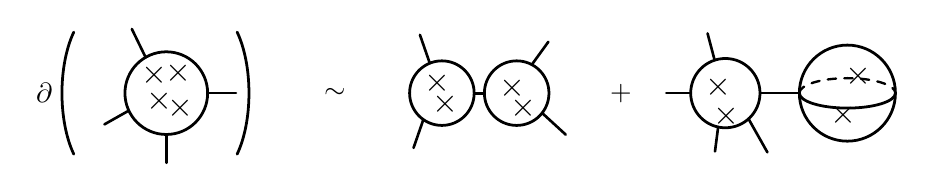
\begin{tikzpicture}[
  x=0.5cm,y=0.5cm,
  line cap=round,
  line join=round,
  >=Latex,
  surf/.style={draw=black,line width=1pt},
  back/.style={draw=black,line width=0.85pt,dashed},
  leg/.style={draw=black,line width=0.95pt},
  seam/.style={draw=black,line width=0.95pt},
  dotstyle/.style={font=\large}
]

% Left: BV operator on one bordered surface
\begin{scope}[shift={(-7.6,0)}]
  \coordinate (C) at (-0.25,0);
  \def\rleft{1.05}
  \draw[surf] (-2.6,1.55) .. controls (-3.0,0.7) and (-3.0,-0.7) .. (-2.6,-1.55);
  \draw[surf] (C) circle [radius=\rleft];
  \draw[surf] (1.55,1.55) .. controls (1.95,0.7) and (1.95,-0.7) .. (1.55,-1.55);

  % exterior legs
  \draw[leg] ($(C)+({\rleft*cos(120)},{\rleft*sin(120)})$) -- ++(-0.35,0.72);
  \draw[leg] ($(C)+({\rleft*cos(205)},{\rleft*sin(205)})$) -- ++(-0.62,-0.35);
  \draw[leg] ($(C)+(0,-\rleft)$) -- ++(0,-0.72);
  \draw[leg] ($(C)+(\rleft,0)$) -- ++(0.72,0);

  % insertions
  \node[dotstyle] at (-0.55, 0.45) {$\times$};
  \node[dotstyle] at ( 0.05, 0.50) {$\times$};
  \node[dotstyle] at (-0.42,-0.20) {$\times$};
  \node[dotstyle] at ( 0.12,-0.38) {$\times$};

  \node at (-3.35,0) {$\partial$};
\end{scope}

% Approximation symbol
\node at (-3.55,0) {$\sim$};

% Middle: splitting into two disks
\begin{scope}[shift={(0.1,0)}]
  \coordinate (A) at (-0.95,0);
  \coordinate (B) at ( 0.95,0);
  \def\rmid{0.82}

  \draw[surf] (A) circle [radius=\rmid];
  \draw[surf] (B) circle [radius=\rmid];
  \draw[surf] ($(A)+(\rmid,0)$) -- ($(B)+(-\rmid,0)$);

  % left component legs
  \draw[leg] ($(A)+({\rmid*cos(112)},{\rmid*sin(112)})$) -- ++(-0.25,0.72);
  \draw[leg] ($(A)+({\rmid*cos(235)},{\rmid*sin(235)})$) -- ++(-0.25,-0.72);

  % right component legs
  \draw[leg] ($(B)+({\rmid*cos(62)},{\rmid*sin(62)})$) -- ++(0.42,0.58);
  \draw[leg] ($(B)+({\rmid*cos(-38)},{\rmid*sin(-38)})$) -- ++(0.60,-0.55);

  % insertions
  \node[dotstyle] at ($(A)+(-0.12, 0.25)$) {$\times$};
  \node[dotstyle] at ($(A)+( 0.10,-0.28)$) {$\times$};
  \node[dotstyle] at ($(B)+(-0.10, 0.12)$) {$\times$};
  \node[dotstyle] at ($(B)+( 0.18,-0.38)$) {$\times$};
\end{scope}

% Plus sign
\node at (3.7,0) {$+$};

% Right: gluing / open-closed propagation
\begin{scope}[shift={(7.7,0)}]
  \coordinate (L) at (-1.35,0);
  \coordinate (R) at ( 1.75,0);
  \def\rdisk{0.88}
  \def\rsphere{1.22}
  \def\requator{0.38}

  % left disk
  \draw[surf] (L) circle [radius=\rdisk];

  % right sphere
  \draw[surf] (R) circle [radius=\rsphere];
  \draw[surf] ($(R)+(-\rsphere,0)$) arc[start angle=180,end angle=360,x radius=\rsphere,y radius=\requator];
  \draw[back] ($(R)+(-\rsphere,0)$) arc[start angle=180,end angle=0,x radius=\rsphere,y radius=\requator];

  % gluing segment
  \draw[seam] ($(L)+(\rdisk,0)$) -- ($(R)+(-\rsphere,0)$);

  % exterior legs
  \draw[leg] ($(L)+(-\rdisk,0)$) -- ++(-0.62,0);
  \draw[leg] ($(L)+({\rdisk*cos(108)},{\rdisk*sin(108)})$) -- ++(-0.18,0.68);
  \draw[leg] ($(L)+({\rdisk*cos(-102)},{\rdisk*sin(-102)})$) -- ++(-0.08,-0.62);
  \draw[leg] ($(L)+({\rdisk*cos(-48)},{\rdisk*sin(-48)})$) -- ++(0.48,-0.85);

  % insertions
  \node[dotstyle] at ($(L)+(-0.18, 0.15)$) {$\times$};
  \node[dotstyle] at ($(L)+( 0.02,-0.58)$) {$\times$};
  \node[dotstyle] at ($(R)+(0.28, 0.42)$) {$\times$};
  \node[dotstyle] at ($(R)+(-0.10,-0.56)$) {$\times$};
\end{scope}

\end{tikzpicture}
\end{center}
\caption{Boundary degeneration at the disk level in the open-closed master equation.}%
\label{fig:disk-level-boundary}
\end{figure}
\end{exm}

\begin{exm}
    Now suppose \(g = 2\) and \(h = 0\). Then the boundary is given in~\Cref{fig:genus-two-closed-boundary} and the corresponding equation is
    \[ Q I_{2,0} + \Delta_c I_{1,0} + \frac{1}{2} \ab\{ I_{1,0}, I_{1,0} \}_c + \ab\{ I_{0,0}, I_{2,0} \}_c = 0. \]

    \begin{figure}[htpb]
    \begin{center}
    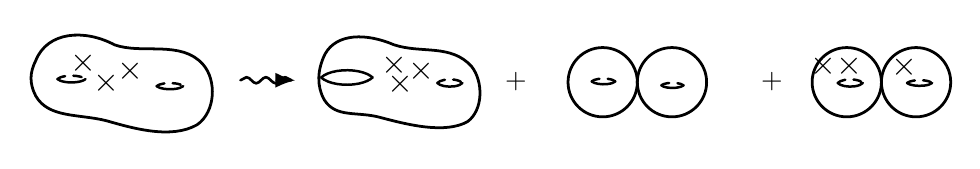
\begin{tikzpicture}[
  x=0.5cm,y=0.5cm,
  line cap=round,
  line join=round,
  >=Latex,
  surf/.style={draw=black,line width=1pt},
  front/.style={draw=black,line width=0.9pt},
  back/.style={draw=black,line width=0.9pt,dashed},
  trans/.style={draw=black,line width=0.95pt,decorate,
    decoration={snake,amplitude=1.1pt,segment length=7pt}},
  ins/.style={font=\large}
]

% Left surface
\begin{scope}[shift={(0,0)}]
  \draw[surf]
    (-2.35,0.55)
      .. controls (-2.05,1.30) and (-1.10,1.35) .. (-0.35,0.95)
      .. controls ( 0.35,0.70) and ( 1.35,1.08) .. ( 1.90,0.45)
      .. controls ( 2.25,0.05) and ( 2.22,-0.75) .. ( 1.75,-1.08)
      .. controls ( 1.10,-1.45) and ( 0.15,-1.18) .. (-0.55,-0.98)
      .. controls (-1.25,-0.80) and (-2.02,-0.92) .. (-2.35,-0.35)
      .. controls (-2.52,-0.02) and (-2.50,0.25) .. (-2.35,0.55)
      -- cycle;

  % genus markers
  \draw[back]  (-1.80, 0.08) arc[start angle=160,end angle=20,x radius=0.38,y radius=0.13];
  \draw[front] (-1.80, 0.08) arc[start angle=200,end angle=340,x radius=0.38,y radius=0.13];
  \draw[back]  ( 0.72,-0.10) arc[start angle=160,end angle=20,x radius=0.36,y radius=0.12];
  \draw[front] ( 0.72,-0.10) arc[start angle=200,end angle=340,x radius=0.36,y radius=0.12];

  % insertions
  \node[ins] at (-1.15, 0.48) {$\times$};
  \node[ins] at (-0.55,-0.02) {$\times$};
  \node[ins] at ( 0.05, 0.28) {$\times$};
\end{scope}

% squiggly arrow
\draw[trans,->] (2.85,0.05) -- (4.25,0.05);

% First term
\begin{scope}[shift={(7.0,0)}]
  \draw[surf]
    (-2.00,0.72)
      .. controls (-1.70,1.25) and (-0.95,1.25) .. (-0.25,0.95)
      .. controls ( 0.45,0.72) and ( 1.20,0.98) .. ( 1.72,0.40)
      .. controls ( 2.02,0.02) and ( 2.02,-0.70) .. ( 1.62,-1.00)
      .. controls ( 1.05,-1.32) and ( 0.10,-1.08) .. (-0.58,-0.90)
      .. controls (-1.18,-0.73) and (-1.72,-0.92) .. (-2.02,-0.45)
      .. controls (-2.22,-0.10) and (-2.20,0.32) .. (-2.00,0.72)
      -- cycle;

  % enlarged left handle
  \draw[front]  (-2.10, 0.12) arc[start angle=155,end angle=25,x radius=0.72,y radius=0.32];
  \draw[front] (-2.10, 0.12) arc[start angle=205,end angle=335,x radius=0.72,y radius=0.32];

  % right handle
  \draw[back]  ( 0.85,-0.02) arc[start angle=160,end angle=20,x radius=0.34,y radius=0.14];
  \draw[front] ( 0.85,-0.02) arc[start angle=200,end angle=340,x radius=0.34,y radius=0.14];

  \node[ins] at (-0.25, 0.42) {$\times$};
  \node[ins] at (-0.08,-0.05) {$\times$};
  \node[ins] at ( 0.45, 0.28) {$\times$};
\end{scope}

\node at (9.85,0.02) {$+$};

% Second term: two circular components
\begin{scope}[shift={(13.0,0)}]
  \draw[surf] (-0.95,0) circle [radius=0.88];
  \draw[surf] ( 0.81,0) circle [radius=0.88];

  \draw[back]  (-1.23,0.02) arc[start angle=160,end angle=20,x radius=0.32,y radius=0.11];
  \draw[front] (-1.23,0.02) arc[start angle=200,end angle=340,x radius=0.32,y radius=0.11];

  \draw[back]  ( 0.54,-0.08) arc[start angle=160,end angle=20,x radius=0.30,y radius=0.10];
  \draw[front] ( 0.54,-0.08) arc[start angle=200,end angle=340,x radius=0.30,y radius=0.10];
\end{scope}

\node at (16.35,0.02) {$+$};

% Third term: two circular components with insertions
\begin{scope}[shift={(19.2,0)}]
  \draw[surf] (-0.95,0) circle [radius=0.88];
  \draw[surf] ( 0.81,0) circle [radius=0.88];

  \draw[back]  (-1.18,-0.02) arc[start angle=160,end angle=20,x radius=0.34,y radius=0.14];
  \draw[front] (-1.18,-0.02) arc[start angle=200,end angle=340,x radius=0.34,y radius=0.14];

  \draw[back]  ( 0.58,-0.02) arc[start angle=160,end angle=20,x radius=0.34,y radius=0.11];
  \draw[front] ( 0.58,-0.02) arc[start angle=200,end angle=340,x radius=0.34,y radius=0.11];

  \node[ins] at (-1.22, 0.40) {$\times \times$};
  \node[ins] at ( 0.51, 0.38) {$\times$};
\end{scope}

\end{tikzpicture}
    \end{center}
    \caption{Boundary degeneration of a genus-two closed surface.}%
    \label{fig:genus-two-closed-boundary}
    \end{figure}
\end{exm}

\begin{exm}
    In the case of an annulus with \(g = 0\) and \(h = 2\), the boundary is given in~\Cref{fig:annulus-four-degenerations} and the corresponding equation is
    \[ Q I_{0,2} + \ab\{ I_{0,0}, I_{0,2} \}_o + \Delta_o I_{0,1} + \frac{1}{2} \ab\{ I_{0,1}, I_{0,1} \}_c + \ab\{ I_{0,0}, I_{0,2} \}_c = 0. \]
    The \(\Delta_o I_{0,1}\) term is the one-loop gauge anomaly, and is cancelled out by the tree-level closed string sector via the Green-Schwarz mechanism.
    \begin{figure}[htpb]
\centering
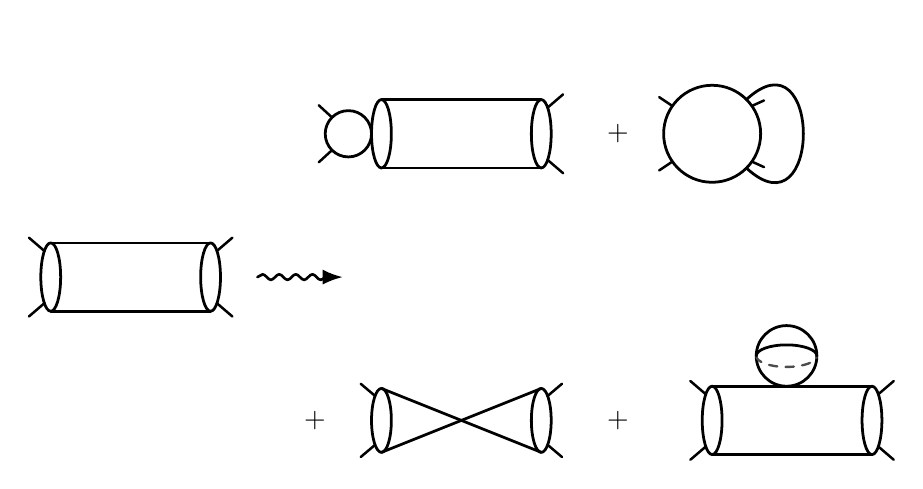
\begin{tikzpicture}[
  x=0.7cm,y=0.7cm,
  line cap=round,
  line join=round,
  >=Latex,
  surf/.style={draw=black,line width=1pt},
  hidden/.style={draw=black!70,dashed,line width=0.85pt},
  leg/.style={draw=black,line width=0.9pt},
  trans/.style={draw=black,line width=0.95pt,decorate,
    decoration={snake,amplitude=1.0pt,segment length=6pt, post=lineto, post length=2pt}}
]

% Non-degenerated annulus
\begin{scope}[shift={(-1.8,-1.05)}]
  \coordinate (L0) at (0,0);
  \coordinate (R0) at (2.9,0);
  \def\rya{0.62}
  \def\rxa{0.18}

  \draw[surf] (L0) ellipse [x radius=\rxa, y radius=\rya];
  \draw[surf] (R0) ellipse [x radius=\rxa, y radius=\rya];
  \draw[surf] ($(L0)+(0,\rya)$) -- ($(R0)+(0,\rya)$);
  \draw[surf] ($(L0)+(0,-\rya)$) -- ($(R0)+(0,-\rya)$);

  % two legs on each boundary circle
  \draw[leg] ($(L0)+({\rxa*cos(130)},{\rya*sin(130)})$) -- ++(-0.28, 0.24);
  \draw[leg] ($(L0)+({\rxa*cos(230)},{\rya*sin(230)})$) -- ++(-0.28,-0.24);
  \draw[leg] ($(R0)+({\rxa*cos(50)},{\rya*sin(50)})$) -- ++( 0.28, 0.24);
  \draw[leg] ($(R0)+({\rxa*cos(-50)},{\rya*sin(-50)})$) -- ++( 0.28,-0.24);
\end{scope}

% Squiggly arrow to degenerations
\draw[trans,->] (1.95,-1.05) -- (3.50,-1.05);

% 1. Boundary disk bubble attached to a cylinder
\begin{scope}[shift={(4.2,1.55)}]
  \coordinate (L) at (0,0);
  \coordinate (R) at (2.9,0);
  \def\ry{0.62}
  \def\rx{0.18}

  % cylinder
  \draw[surf] (L) ellipse [x radius=\rx, y radius=\ry];
  \draw[surf] (R) ellipse [x radius=\rx, y radius=\ry];
  \draw[surf] ($(L)+(0,\ry)$) -- ($(R)+(0,\ry)$);
  \draw[surf] ($(L)+(0,-\ry)$) -- ($(R)+(0,-\ry)$);

  % boundary bubble
  \draw[surf] (-0.60,0) circle [radius=0.42];

  % two legs on the disk bubble
  \draw[leg] ({-0.60 + 0.42*cos(135)},{0.42*sin(135)}) -- ++(-0.24, 0.22);
  \draw[leg] ({-0.60 + 0.42*cos(225)},{0.42*sin(225)}) -- ++(-0.24,-0.22);

  % two legs on the right boundary circle
  \draw[leg] ($(R)+({\rx*cos(50)},{\ry*sin(50)})$) -- ++( 0.28, 0.24);
  \draw[leg] ($(R)+({\rx*cos(-50)},{\ry*sin(-50)})$) -- ++( 0.28,-0.24);
\end{scope}

% 2. Circle with loop
\begin{scope}[shift={(10.2,1.55)}]
  \draw[surf] (0,0) circle [radius=0.88];
  \draw[surf]
    (0.62,0.62)
      .. controls (2.00,1.90) and (2.00,-1.90) .. (0.62,-0.62);

  % two legs on the left hemisphere
  \draw[leg] ({0.88*cos(145)},{0.88*sin(145)}) -- ++(-0.24, 0.16);
  \draw[leg] ({0.88*cos(215)},{0.88*sin(215)}) -- ++(-0.24,-0.16);

  % two legs on the right hemisphere, staying inside the loop
  \draw[leg] ({0.88*cos(35)},{0.88*sin(35)}) -- ++(0.22, 0.10);
  \draw[leg] ({0.88*cos(-35)},{0.88*sin(-35)}) -- ++(0.22,-0.10);
\end{scope}

% 3. Two disks: circle-to-empty composed with empty-to-circle
\begin{scope}[shift={(4.2,-3.65)}]
  \coordinate (N) at (1.45,0);
  \coordinate (CL) at (0,0);
  \coordinate (CR) at (2.9,0);
  \def\ry{0.58}
  \def\rx{0.18}

  \draw[surf] (CL) ellipse [x radius=\rx, y radius=\ry];
  \draw[surf] (CR) ellipse [x radius=\rx, y radius=\ry];

  \draw[surf] ($(CL)+(0,\ry)$) -- (N);
  \draw[surf] ($(CL)+(0,-\ry)$) -- (N);
  \draw[surf] (N) -- ($(CR)+(0,\ry)$);
  \draw[surf] (N) -- ($(CR)+(0,-\ry)$);

  % two legs on each boundary circle
  \draw[leg] ($(CL)+({\rx*cos(130)},{\ry*sin(130)})$) -- ++(-0.26, 0.22);
  \draw[leg] ($(CL)+({\rx*cos(230)},{\ry*sin(230)})$) -- ++(-0.26,-0.22);
  \draw[leg] ($(CR)+({\rx*cos(50)},{\ry*sin(50)})$) -- ++( 0.26, 0.22);
  \draw[leg] ($(CR)+({\rx*cos(-50)},{\ry*sin(-50)})$) -- ++( 0.26,-0.22);
\end{scope}

% 4. Sphere bubble attached to the cylinder along the bulk
\begin{scope}[shift={(10.2,-3.65)}]
  \coordinate (L) at (0,0);
  \coordinate (R) at (2.9,0);
  \def\ry{0.62}
  \def\rx{0.18}
  \coordinate (A) at (1.35,\ry); % attachment point

  % cylinder
  \draw[surf] (L) ellipse [x radius=\rx, y radius=\ry];
  \draw[surf] (R) ellipse [x radius=\rx, y radius=\ry];
  \draw[surf] ($(L)+(0,\ry)$) -- ($(R)+(0,\ry)$);
  \draw[surf] ($(L)+(0,-\ry)$) -- ($(R)+(0,-\ry)$);

  \def\rs{0.55}
  % sphere bubble
  \coordinate (S) at ($(A)+(0,\rs)$);
  \draw[surf] (S) circle [radius=\rs];
  \draw[hidden] ($(S)+(-\rs,0)$) arc[start angle=180,end angle=360,x radius=\rs,y radius=0.20];
  \draw[surf]   ($(S)+(-\rs,0)$) arc[start angle=180,end angle=0,x radius=\rs,y radius=0.20];

  % two legs on each boundary circle
  \draw[leg] ($(L)+({\rx*cos(130)},{\ry*sin(130)})$) -- ++(-0.28, 0.24);
  \draw[leg] ($(L)+({\rx*cos(230)},{\ry*sin(230)})$) -- ++(-0.28,-0.24);
  \draw[leg] ($(R)+({\rx*cos(50)},{\ry*sin(50)})$) -- ++( 0.28, 0.24);
  \draw[leg] ($(R)+({\rx*cos(-50)},{\ry*sin(-50)})$) -- ++( 0.28,-0.24);
\end{scope}

% Row separators
\node at (8.5, 1.55) {$+$};
\node at (8.5,-3.65) {$+$};
\node at (3.0, -3.65) {$+$};

\end{tikzpicture}
\caption{Four boundary strata in the degeneration of the annulus.}
\label{fig:annulus-four-degenerations}
\end{figure}
\end{exm}

\begin{thm}[Costello-Li]
    On \(X = \C^n\), start with:
    \begin{itemize}
        \item Holomorphic Chern-Simons theory on \( \Omega^{0, \bullet}(X) \otimes \mf{gl}_{N\mid N}\). This is necessary because \(\on{Tr}_{\mf{gl}_N}(\bigcirc) = N \neq 0\), but \(\on{Tr}_{\mf{gl}_{N \mid N}}(\bigcirc) = 0\).
        \item A first order deformation.
    \end{itemize}
    There exists a canonical quantization \( \{ I_{g,h} \}\) for all \(g,h\) which satisfies the open-closed master equation.
\end{thm}

\begin{rmk}
    These quantizations glue to any local Calabi-Yau with a non-trivial \(\C^{\times}\)-action.
\end{rmk}

\begin{rmk}
    The open-closed B-model which is BCOV coupled to holomorphic Chern-Simons theory is UV finite on any Calabi-Yau manifold (assumed to be K\"ahler).
\end{rmk}


\end{document}

%%% Local Variables:
%%% mode: latex
%%% TeX-master: t
%%% End:
